\documentclass{article}
\usepackage{graphicx} % Required for inserting images
\usepackage{svg} % Makes it possible to include svg-images
\usepackage{cite}
\usepackage[a4paper, total={6in, 8in}]{geometry}
\usepackage{float}
\usepackage{makecell}
\usepackage{colortbl}
\usepackage{listings}
\usepackage[colorlinks=true,allcolors=black]{hyperref}
\usepackage[british]{babel}     % Defining UK English as language. This will among other things ensure that dates are displayed as 24/03/1997 rather than 03/24/1997 in the bibliography.
\addto\extrasbritish{   % Change naming of different functions, e.g. figure references.
    \renewcommand*\contentsname{Table of Contents}  % Rename table of contents
    \renewcommand{\listfigurename}{List of Figures} % Rename list of figures
    \renewcommand{\listtablename}{List of Tables}   % Rename list of tables
    \def\equationautorefname{Equation}              % Autoref-name for equations
    \def\figureautorefname{Figure}                  % Autoref-name for figures
    \def\tableautorefname{Table}                    % Autoref-name for tables
    \def\sectionautorefname{Section}                % Autoref-name for sections
    \def\subsectionautorefname{Subsection} % Autoref-name for subsections
    \def\subsubsectionautorefname{Subsection} % Autoref-name for subsubsections
}

\lstdefinestyle{aimspiceStyle}{
    language=Verilog,
    basicstyle=\small\ttfamily,
    commentstyle=\color{green},
    keywordstyle=,
    numberstyle=\tiny\color{gray},
    numbers=left,
    numbersep=5pt,
    breaklines=true,
    frame=lines,
    backgroundcolor=\color{lightgray!20}, % Adjust the percentage for a lighter shade
}

\lstdefinestyle{verilogStyle}{
    language=Verilog,     % Set the language to Verilog
    basicstyle=\small\ttfamily,
    commentstyle=\color{green},
    keywordstyle=\color{blue},
    numberstyle=\tiny\color{gray},
    numbers=left,
    numbersep=5pt,
    breaklines=true,
    frame=lines,
    backgroundcolor=\color{lightgray!20}, % Lighter background color
}



\begin{document}

\begin{titlepage}
\vbox{ }
\vbox{ }
\begin{center}
% Upper part of the page
\includesvg[width=\textwidth]{Figures/logo.svg}\\[1cm]
\textsc{\LARGE TFE4152 Design of Integrated Circuits}\\[1cm]
\textsc{\Large Term project fall 2023}\\[0.5cm]
\vbox{ }

% Title
\HRule \\[0.4cm]
{ \huge \bfseries Design \& Test of a \\Multiply-Accumulate unit}\\[0.4cm] %TODO: replace "TITLE" with some project title, e.g. "Design of a Multiply Accumulate Unit"
\HRule \\[1.5cm]

% Author
\large
\emph{Authors:}\\
Einar Bergslid \& Kristian Gøystdal %TODO: Replace this line with your names
\vfill

\end{center}
\end{titlepage}


\section{Introduction}
\label{sec:introduction}

The Multiply-Accumulate (MAC) unit plays a crucial role in digital signal processing and various computational tasks, especially in artificial intelligence. In this project, we aim to design an efficient and reliable MAC unit using the gpdk 90nm technology. This technology ensures compatibility with real-world electronic circuits. Our goal is not only to meet given specifications but also to gain a deeper understanding of digital circuitry principles. 

The design of the MAC unit has to comply to certain specifications, given in detail in the project description\cite{project_description}. A short summary of the given specifications is shown in table~\ref{tab:specifications}.

\begin{table}[H]
\caption{Given specifications for the MAC unit}
\label{tab:specifications}
\centering
\begin{tabular}{|c|l|}
\hline
\rowcolor[HTML]{C0C0C0} 
 Specification & Description \\ \hline
 1 & The gpdk 90nm technology is to be used \\ \hline
 2 & The circuit should consist of two subsystems: FSM and MAC \\ \hline
 3 & The FSM has three inputs: Reset, CLK and Run  \\ \hline
 4 & The FSM’s state should only be updated at the positive edge of the clock \\ \hline
 5 & All binary numbers are unsigned \\ \hline
 6 & The MAC unit has two 2-bit inputs A and B \\ \hline
 7 & \makecell[l]{The MAC unit must multiply A and B and add the product\\ to the currently stored value}  \\ \hline
 8 & \makecell[l]{The accumulated value must be stored in a 8-bit register in the MAC unit,\\ and be updated at each positive edge of the clock} \\ \hline
 9 & The MAC unit should output the accumulated 8-bit value \\ \hline
 10 & Gate lengths must be $\le$ 300 nm \\ \hline
 10 & Gate widths must be $\le$ 1500 nm \\ \hline
 11 & The upper limit for any supply voltage is 1.0 V \\ \hline
 11 & No logic gate can have a fan-in of more than 4 \\ \hline
\end{tabular}
\end{table}

In addition to the given criteria above, the static power consumption of the circuit should be considered. The goal is to create a low power MAC unit, i.e. a MAC unit that consumes little static power. This means that static power consumption should be considered when choosing circuit topology, transistor dimensions, supply voltage, etc. and when designing the FSM. The verification of funtionality and power consumption is discussed in section~\ref{sec:results}.
\newpage
\section{Theory}
\label{sec:theory}

The Multiply accumulate circuit can be divided into different subsystems. In this section we are going to explain the functions of each subsystem and create a circuit design to implement in later sections. In figure \ref{fig:blokk} the different subsystems are shown and how they connect. 

\begin{figure}[H]
    \centering
    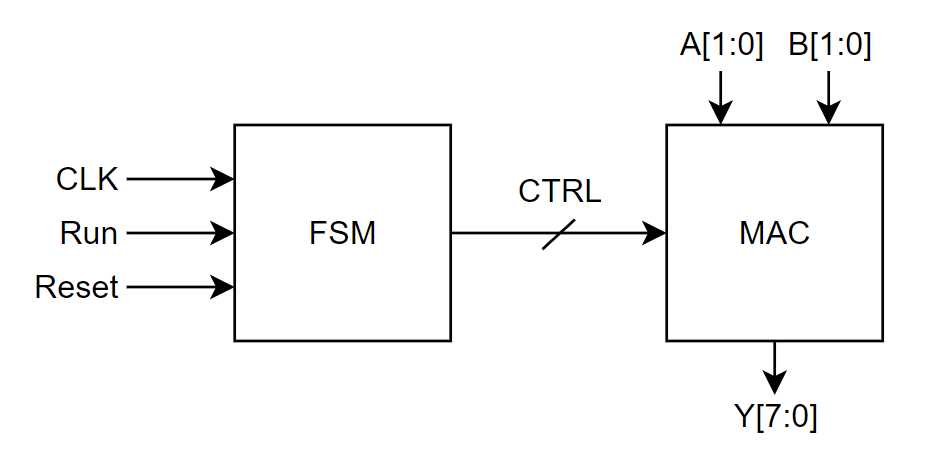
\includegraphics[width=0.7\textwidth]{Figures/Blokk.png}
    \caption{An overview of the complete system.}
    \label{fig:blokk}
\end{figure}


\subsection{Finite State Machine}
\label{subsec:fsm_theory}

A finite state machine (FSM) is a model used to describe a system with a finite number of states. It operates by transitioning from one state to another in response to inputs, following a defined set of rules. FSMs consist of:

\begin{enumerate}
    \item \textbf{States}: These represent distinct conditions or configurations that the system can be in. Transitions occur between states based on inputs.
    
    \item \textbf{Transitions}: These are directed connections between states, triggered by specific input conditions. Transitions determine the movement from one state to another.
    
    \item \textbf{Inputs}: These are external signals that trigger state transitions. Inputs influence the behavior of the FSM.
    
    \item \textbf{Outputs}: FSMs may generate outputs in response to inputs and state transitions. Outputs convey information about the current state or operation of the system.
\end{enumerate}

\noindent
FSMs can be classified into two main types:

\begin{enumerate}
    \item \textbf{Mealy Machine}: In a Mealy machine, the outputs depend on both the current state and the input. The output is produced immediately after an input is received and a state transition occurs. 
    
    \item \textbf{Moore Machine}: In a Moore machine, the outputs depend only on the current state. The output is associated with the state itself, so it changes only after a state transition.
\end{enumerate}

A general overview of the functionality is shown in figure~\ref{fig:general_fsm}.

\begin{figure}[H]
    \centering
    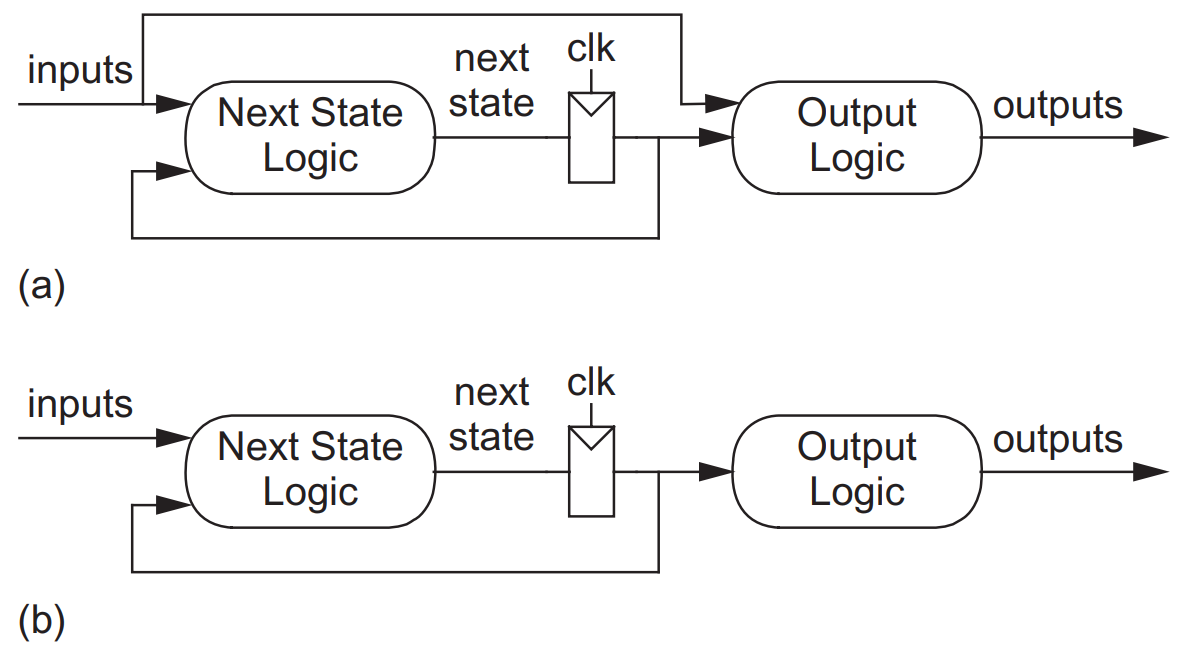
\includegraphics[width=0.8\textwidth]{Figures/general fsm diagrams.png}
    \caption{a: Mealy FSM b: Moore FSM \cite{CMOS_VLSI_design}}
    \label{fig:general_fsm}
\end{figure}


\noindent
A certain design procedure can be used for the design of FSMs~\cite{digital_design}:

\begin{enumerate}
  \item From the word description and specifications of the desired operation, derive a state diagram for the circuit.
  \item Reduce the number of states if necessary.
  \item Assign binary values to the states.
  \item Obtain a binary-coded state table.
  \item Choose the type of flip-flops to be used.
  \item Derive the simplified flip-flop input equations and output equations.
  \item Draw the logic diagram.
\end{enumerate}


\subsection{MAC}
\label{subsec:MAC_theory}

\begin{equation}
    \label{eq:mac}
    C \leftarrow C + (A \cdot B)
\end{equation}

The MAC unit will receive two 2-bit inputs, A and B, which will be multiplied and added to C, as shown in \ref{eq:mac}. This should happen every rising edge of the clock. The MAC unit consist of a multiplier, an adder and an accumulator. The layout of the MAC is shown in figure \ref{fig:mac-blokk}. 

\begin{figure}[htpb]
    \centering
    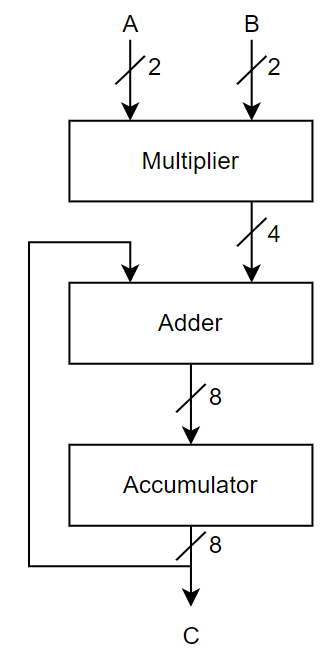
\includegraphics[width=0.3\textwidth]{Figures/mac-blokk.png}
    \caption{Layout of MAC unit}
    \label{fig:mac-blokk}
\end{figure}

\subsubsection{Multiplier}
The multiplier takes in A and B, two 2 bits inputs, and multiply them. The value of A times B can't be higher than 9, which means that the output of the multiplier has to be at least 4 bits. 

\subsubsection{Adder}
As shown in figure \ref{fig:mac-blokk}, the adder has to take the sum of a 4-bit number (A) and a 8-bit number (B). Since the multiplier only outputs a 4-bit number, the four most significant bits of A will always be set to low. The design of an 8-bit adder is shown in figure \ref{fig:adder-blokk}. The figure shows two 8-bit numbers A and B, and their sum S with a carry $C_O$. 

\begin{figure}[H]
    \centering
    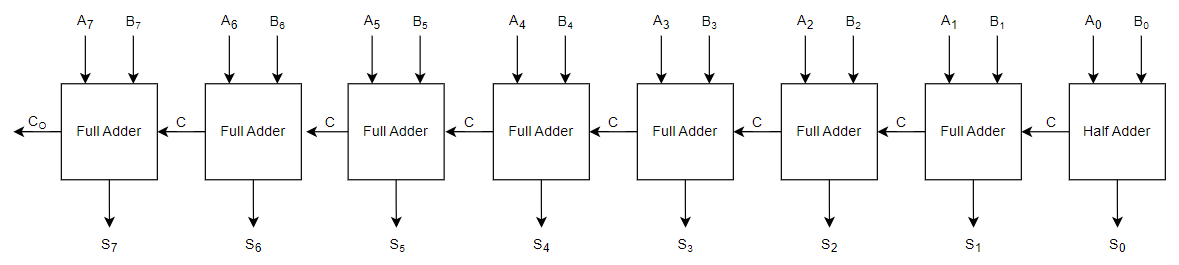
\includegraphics[width=0.8\textwidth]{Figures/8bitadder.png}
    \caption{8-bit adder}
    \label{fig:adder-blokk}
\end{figure}


\subsubsection{Accumulator}
The accumulator is an 8-bit register with some control signals, set (S) and reset (R). These controll signals are received from the Final State Machine (FSM). The registers are D-flip flops, which only change the stored value at the rising edge of the clock signal. 

\begin{figure}[H]
    \centering
    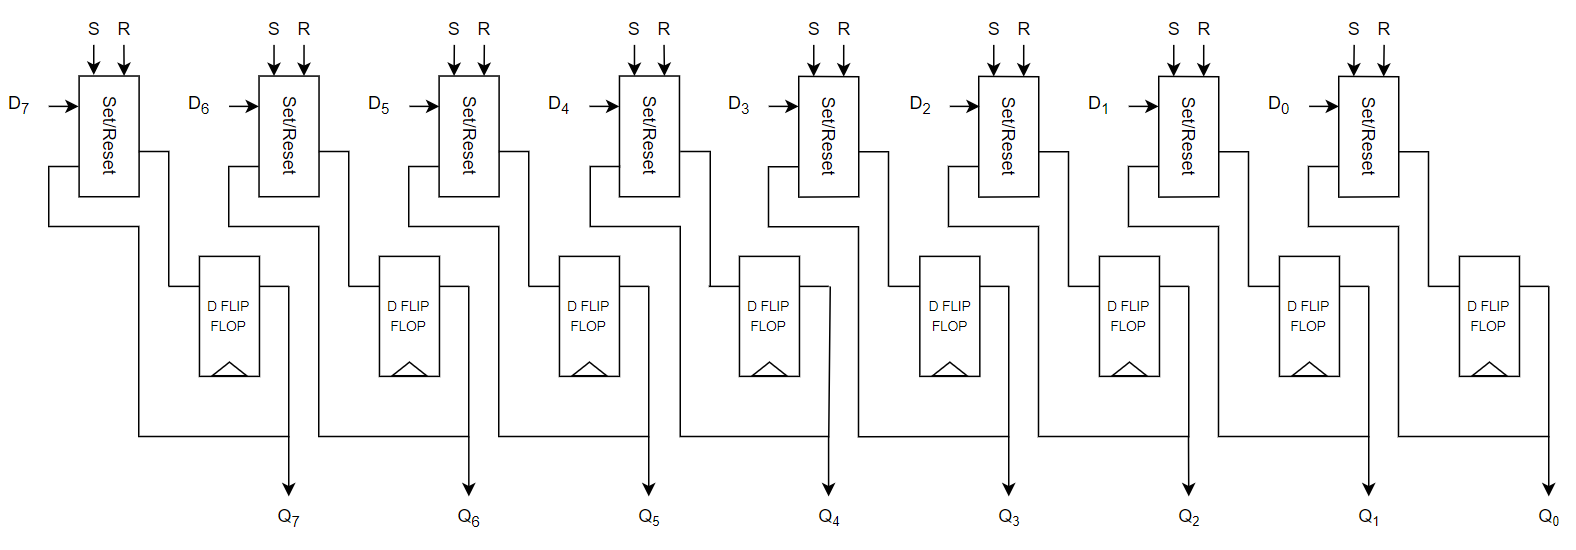
\includegraphics[width=0.9\textwidth]{Figures/8bitRegister.png}
    \caption{8 bit register}
    \label{fig:8bitregister}
\end{figure}


% The theory section should contain background theory relevant for the reader in order to understand the rest of your report. Assume that the reader is yourselves at the start of the semester (before you had learnt anything from this course) and include theory accordingly. Keep in mind that this section should only include theory relevant to the project and the report, it is not meant as a place to show off everything you have ever learnt. 

\subsection{Static Power Consumption}
\label{subsec:low_power}

One can consider many aspects of a circuit design to affect the static power consumption. As the transistor technology is given by the spesification table (\ref{tab:specifications})


When  the static power consumption for the TT and FF corner, we look at a state where the CLK is not running and the inputs, D, S and R, are set to low. The static power consumption is calculated by taking the current in the $V_{DD}$ node and multiplying it with the $V_{DD}$, as shown in equation \ref{eq:power}.

\begin{equation}
    \label{eq:power}
    P = I \cdot V_{DD}
\end{equation}

\subsection{Other theory}\label{subsec:theory_aSubsection}

**Insert other relevant theory here**


% When you in later sections apply any of the theory you can refer back to this section. To make it easier for the reader to understand which part you are referring back to, it can be a good idea to divide your sections into subsections (e.g. one subsection per topic). This also makes it easier to read.

% Use equations, figures and tables to help get your message across. All figures/tables/equations should be referenced in the text, as they are there to help you tell your story. Remember to cite your references \cite{example}.
\section{Method}
\label{sec:method}

In this section we explain how be implement and test the two systems, using AIMSpice to create and test a 1-bit register, and Verilog to create the full circuit. 

\subsection{MAC design}
\label{subsec:circuitDesign}

In this section we will look on how to implement the different subsystems of the MAC unit. The designs are shown at a logic gate level as that is used for both the AIMSpice and Verilog implementation. 

\subsubsection{Multiplier} 

A 2-bit multiplier could be designed like shown in \autoref{fig:multiplier}, which takes in A and B as two 2-bits inputs and outputs a 4-bit signal O. 

\begin{figure}[H]
    \centering
    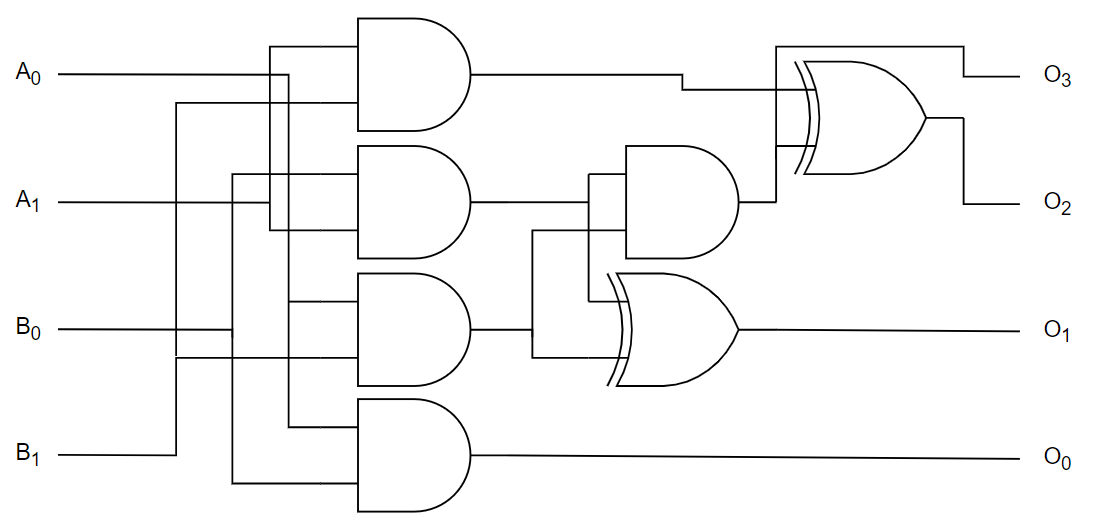
\includegraphics[width=0.8\textwidth]{Figures/multiplier.png}
    \caption{Possible design of multiplier}
    \label{fig:multiplier}
\end{figure}

\subsubsection{Adder}

The design of an 8-bit adder is shown in \autoref{fig:adder-blokk}. The figure shows two 8-bit numbers A and B, and their sum S with a carry $C_O$. 

\begin{figure}[H]
    \centering
    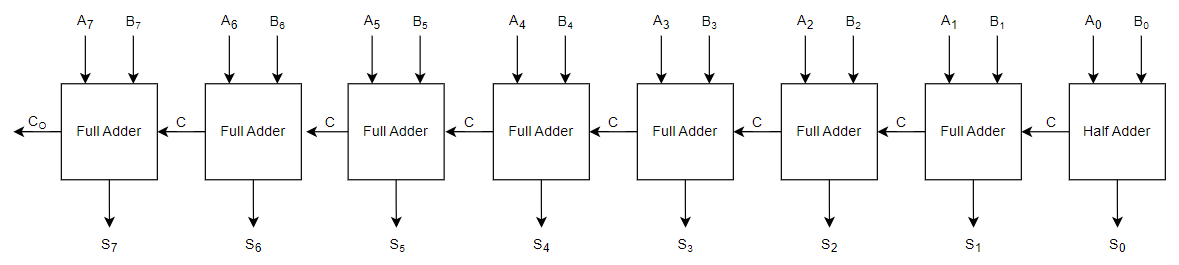
\includegraphics[width=\textwidth]{Figures/8bitadder.png}
    \caption{8-bit adder}
    \label{fig:adder-blokk}
\end{figure}

The circuit for the half and full adder is shown in \autoref{fig:halfadder} and \ref{fig:fulladder}. 

\begin{figure}[H]
\begin{minipage}{0.4\textwidth}
    \centering
    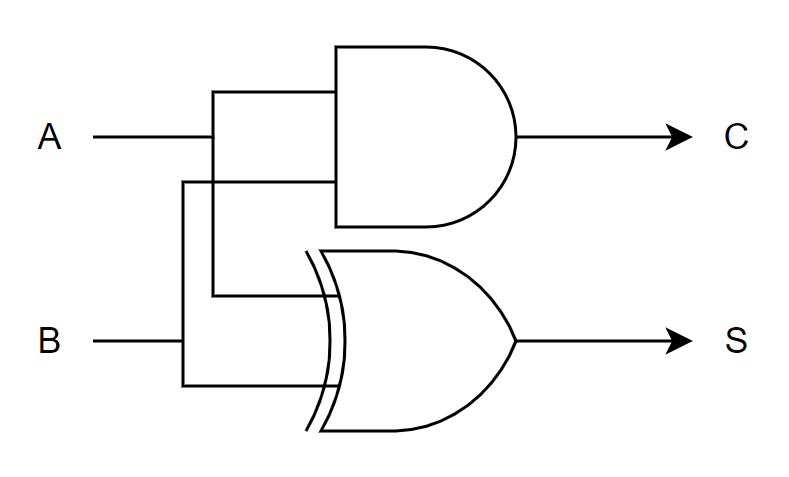
\includegraphics[width=\linewidth]{Figures/halfadder.png}
    \caption{Half adder}
    \label{fig:halfadder}
\end{minipage}
\begin{minipage}{0.6\textwidth}
    \centering
    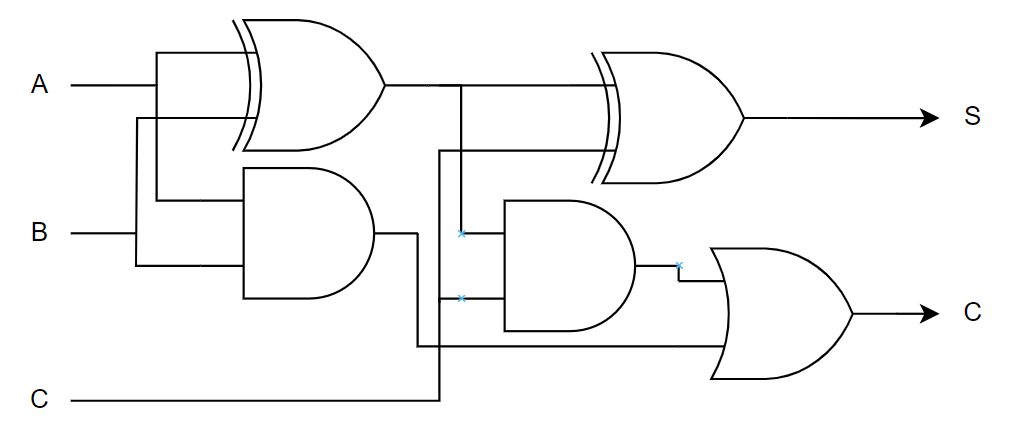
\includegraphics[width=\linewidth]{Figures/fulladder.png}
    \caption{Full adder}
    \label{fig:fulladder}
\end{minipage}
\end{figure}


\subsubsection{Accumulator}
\label{subsubsec:accumulator}
The accumulator is an 8-bit register with some control signals, that is received from the FSM. 

\begin{figure}[H]
    \centering
    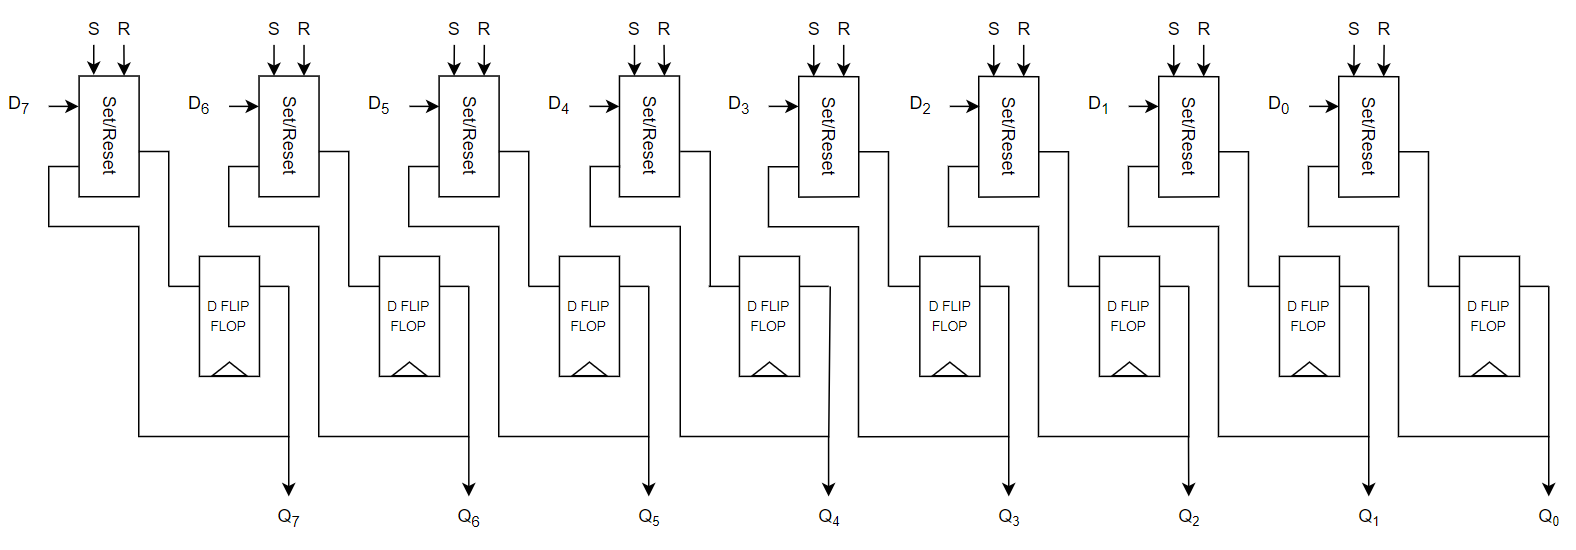
\includegraphics[width=0.9\textwidth]{Figures/8bitRegister.png}
    \caption{8 bit register}
    \label{fig:8bitregister}
\end{figure}

As shown in \autoref{fig:8bitregister}, the accumulator consists of a D-Flip-Flop and a control circuit. These are implemented as shown in \autoref{fig:dflipflop} and \ref{fig:setreset} respectively.

\begin{figure}[H]
    \centering
    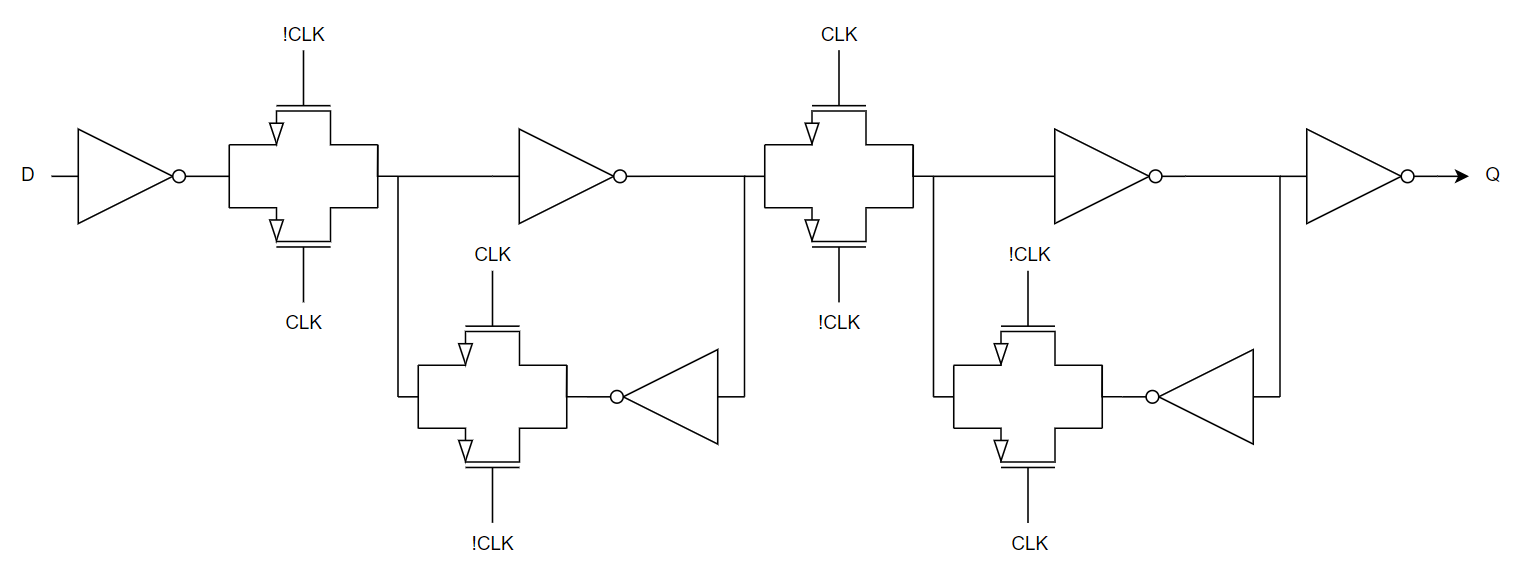
\includegraphics[width=\textwidth]{Figures/D_Flip_Flop.png}
    \caption{D-flip flop}
    \label{fig:dflipflop}
\end{figure}

\begin{figure}[H]
    \centering
    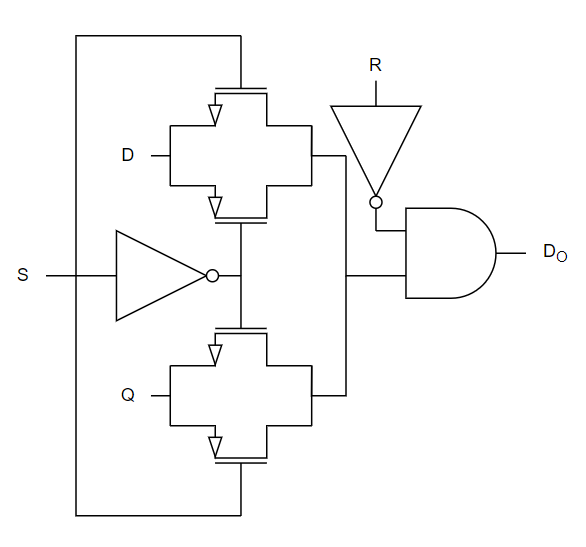
\includegraphics[width=0.4\textwidth]{Figures/setReset.png}
    \caption{Circuit for controlling register}
    \label{fig:setreset}
\end{figure}

\subsection{FSM design}

The FSM was designed according to the project description and the design procedure given in \autoref{subsec:fsm_theory}. Both a Mealy and a Moore FSM design has been considered. The Mealy state machine resulted in 4 states needed and the Moore machine resulted in 8 states needed, requiring an additional state register and more combinatorial logic. The final design was subsequently chosen to be a Mealy FSM, to minimize the amount of transistors. The state diagram derived from the text description is shown in \autoref{fig:fsm_diagram}. To be able to hold four different states, one pause state and three different run states, the FSM needs a 2-bit register, with at least a reset function. 

\begin{figure}[H]
    \centering
    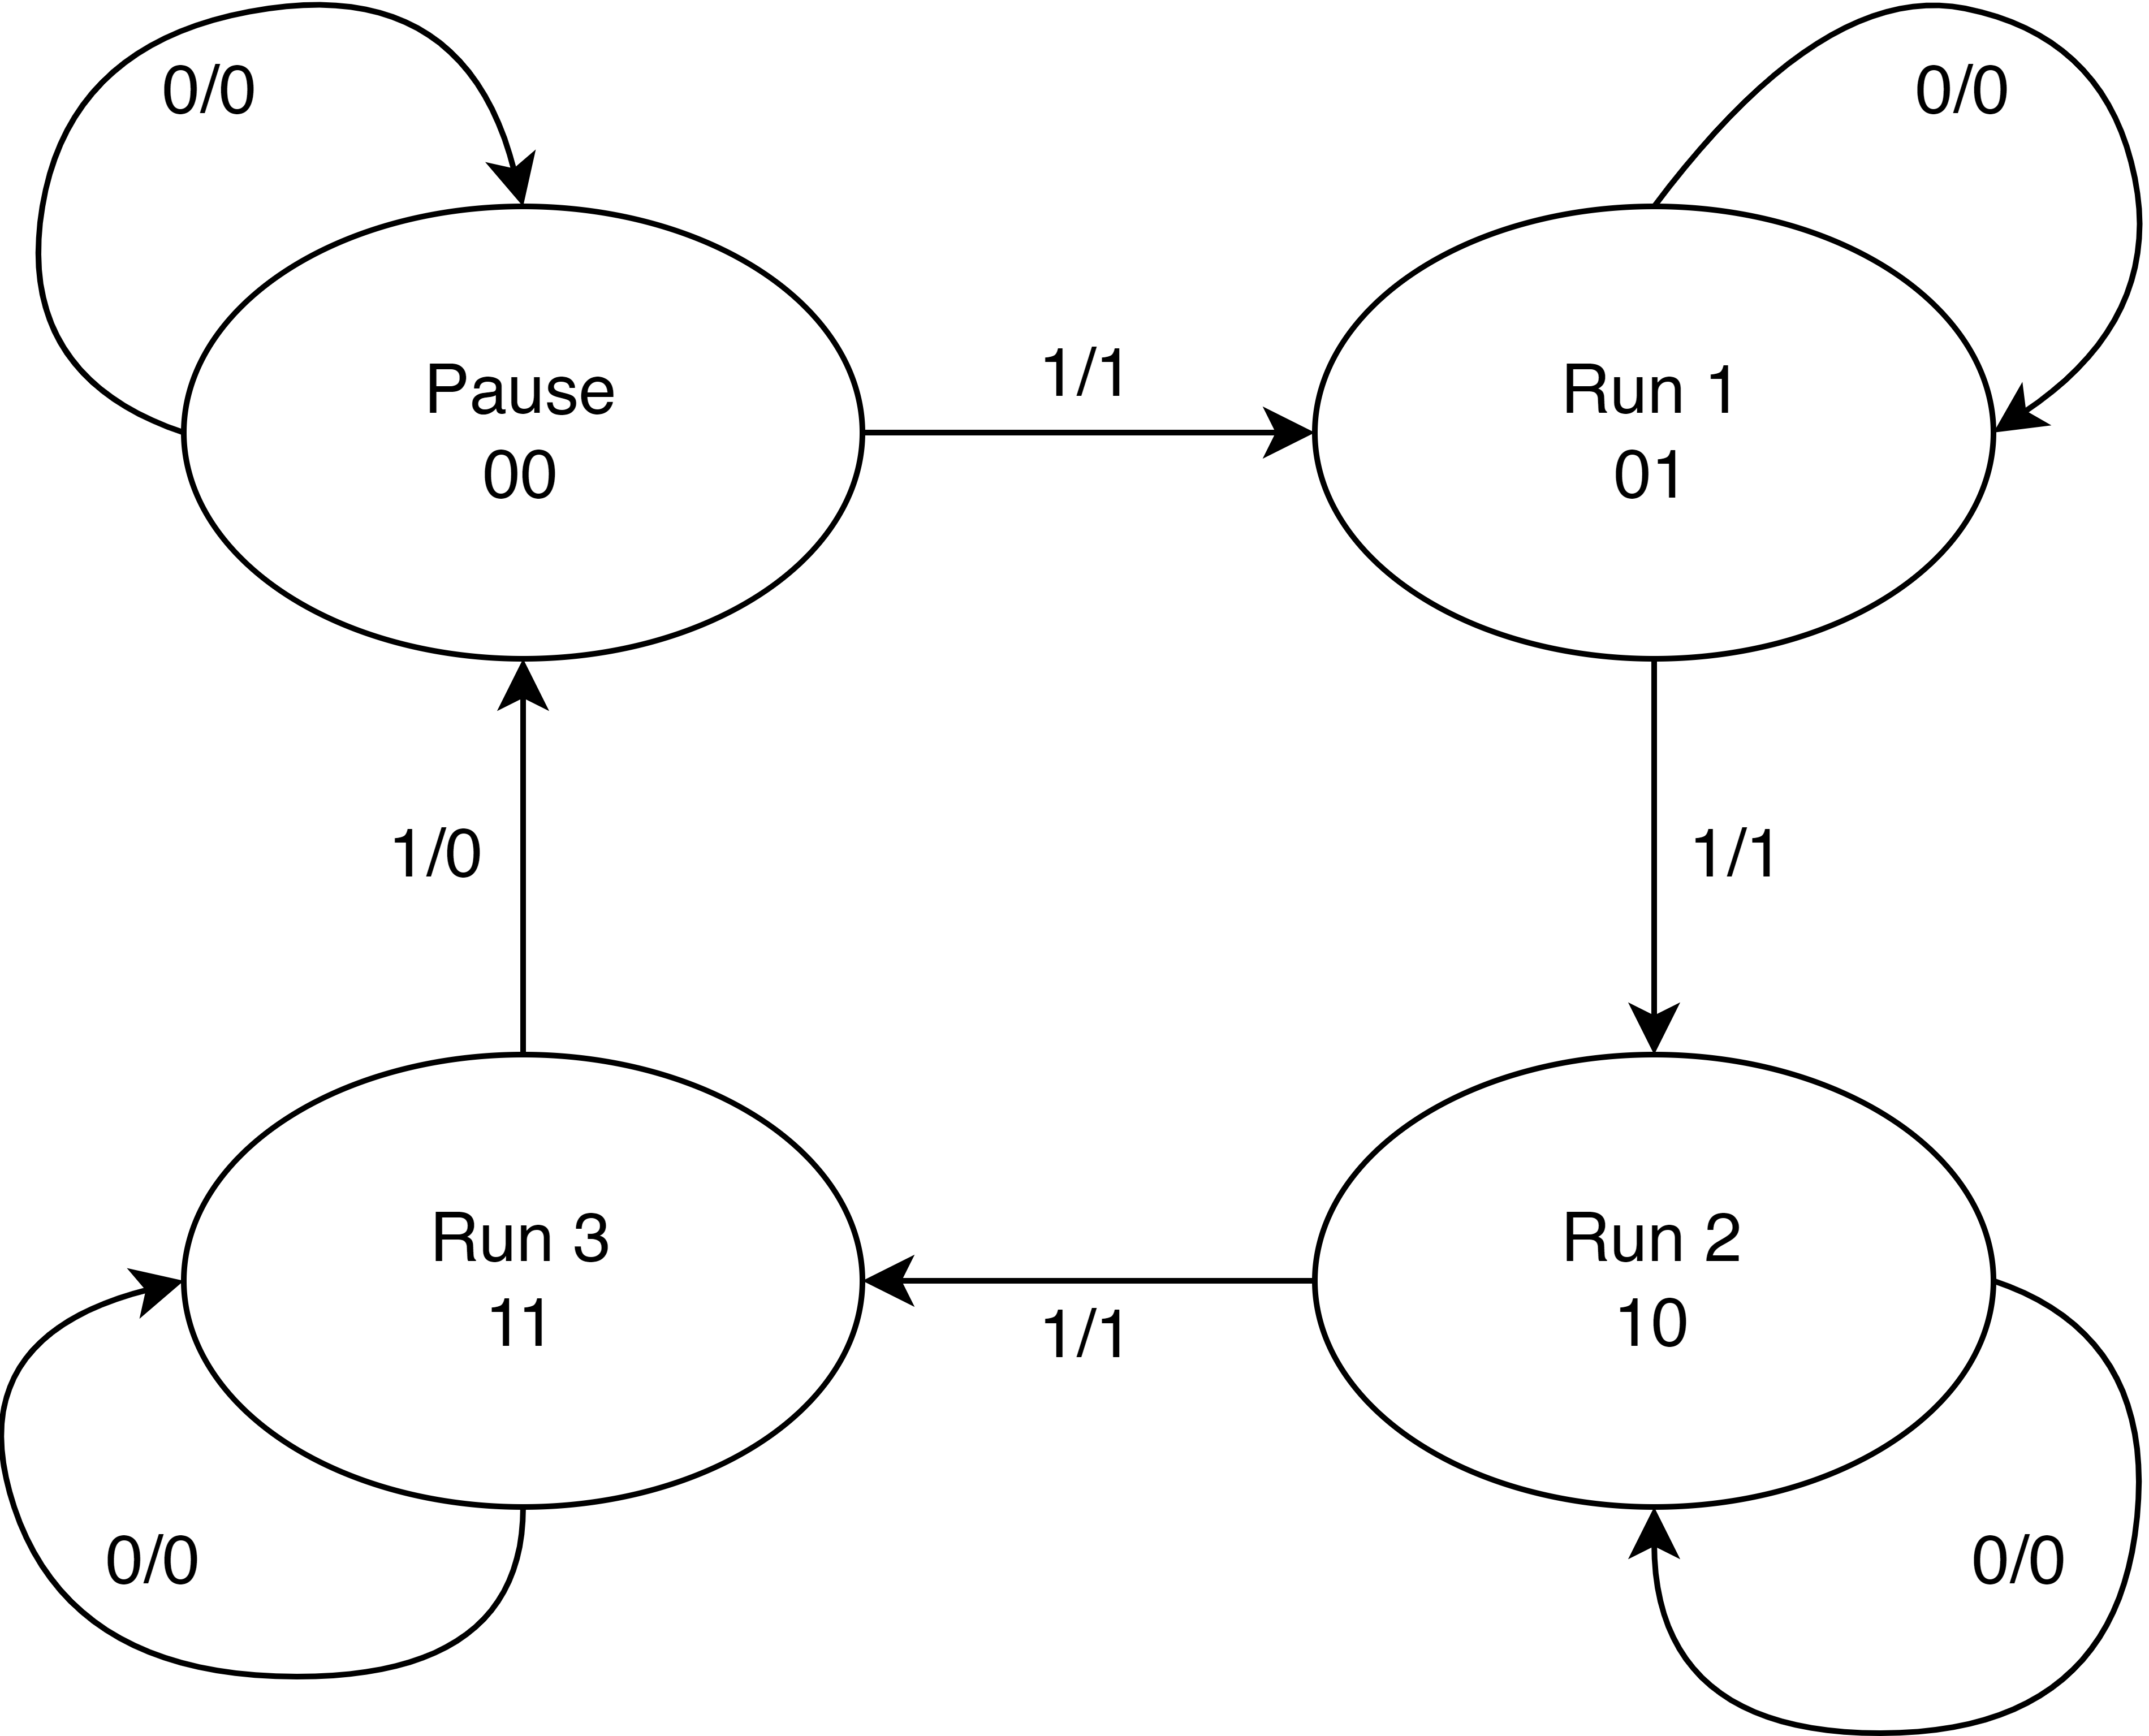
\includegraphics[width=0.8\textwidth]{Figures/FSM-diagram.png}
    \caption{FSM state diagram}
    \label{fig:fsm_diagram}
\end{figure}

Three input signals are given by the project description~\cite{project_description}, Reset, CLK and Run. The CLK-signal
will only be used to time the sequential logic in the FSM and passed on to the MAC unit without
further modification. The CLK signal is therefore not considered an input-signal here in the sense that is not used in the next-state or output-logic in the FSM (\autoref{fig:general_fsm}). The reset input signal $I_1$ is only used to reset the state register to the pause-state ''00'' and passed on to the MAC unit as $CTRL_1$ without further modification. The combinatorial part of the FSM is here only dependent on the current state ($C_1$ and $C_0$) and the Run input signal $I_0$. The outputs of the FSM are the next state signals $N_1$ and $N_0$, and the Reset and Run control signals $CTRL_1$ and $CTRL_0$. From the state diagram, we can write up the state table, \autoref{tab:state_table}. Note that $CTRL_1$ only is dependent on $I_1$ and that this does not require combinatorial logic.

\begin{table}[H]
\caption{State table for the FSM}
\label{tab:state_table}
\centering
\begin{tabular}{|l|l|l|l|l|l||l|l|}
\hline
\rowcolor[HTML]{C0C0C0} 
$C_1$ & $C_0$ & $I_0$ & $N_1$ & $N_0$ & $CTRL_0$ & $I_1$ & $CTRL_1$\\
\hline
0  & 0  & 0  & 0   & 0   & 0 & 1 & 1\\ 
\hline
0  & 0  & 1  & 0   & 1   & 1 & 0 & 0\\ 
\hline
0  & 1  & 0  & 0   & 1   & 0 \\ 
\cline{1-6}
0  & 1  & 1  & 1   & 0   & 1 \\ 
\cline{1-6}
1  & 0  & 0  & 1   & 0   & 0 \\ 
\cline{1-6}
1  & 0  & 1  & 1   & 1   & 1 \\ 
\cline{1-6}
1  & 1  & 0  & 1   & 1   & 0 \\ 
\cline{1-6}
1  & 1  & 1  & 0   & 0   & 0 \\ 
\cline{1-6}

\end{tabular}
\end{table}

\noindent
The logic expression for each of the outputs of the combinatorial logic can be written down and simplified to \autoref{eq:comb_eq_1}, \ref{eq:comb_eq_2}, \ref{eq:comb_eq_3} and \ref{eq:comb_eq_4}.

\begin{equation}
\label{eq:comb_eq_1}
    CTRL_0 = I_0\cdot(\overline{C_1 \cdot C_0})
\end{equation}

\begin{equation}
\label{eq:comb_eq_2}
    N_0 = C_0 \oplus I_0
\end{equation}

\begin{equation}
\label{eq:comb_eq_3}
    N_1 = C_1 \oplus (C_0 \cdot I_0)
\end{equation}

\begin{equation}
\label{eq:comb_eq_4}
    CTRL_1 = I_1
\end{equation}

From the boolean equations, we can draw up the logic diagram shown in \autoref{fig:fsm_logic_diagram}.

\begin{figure}[H]
    \centering
    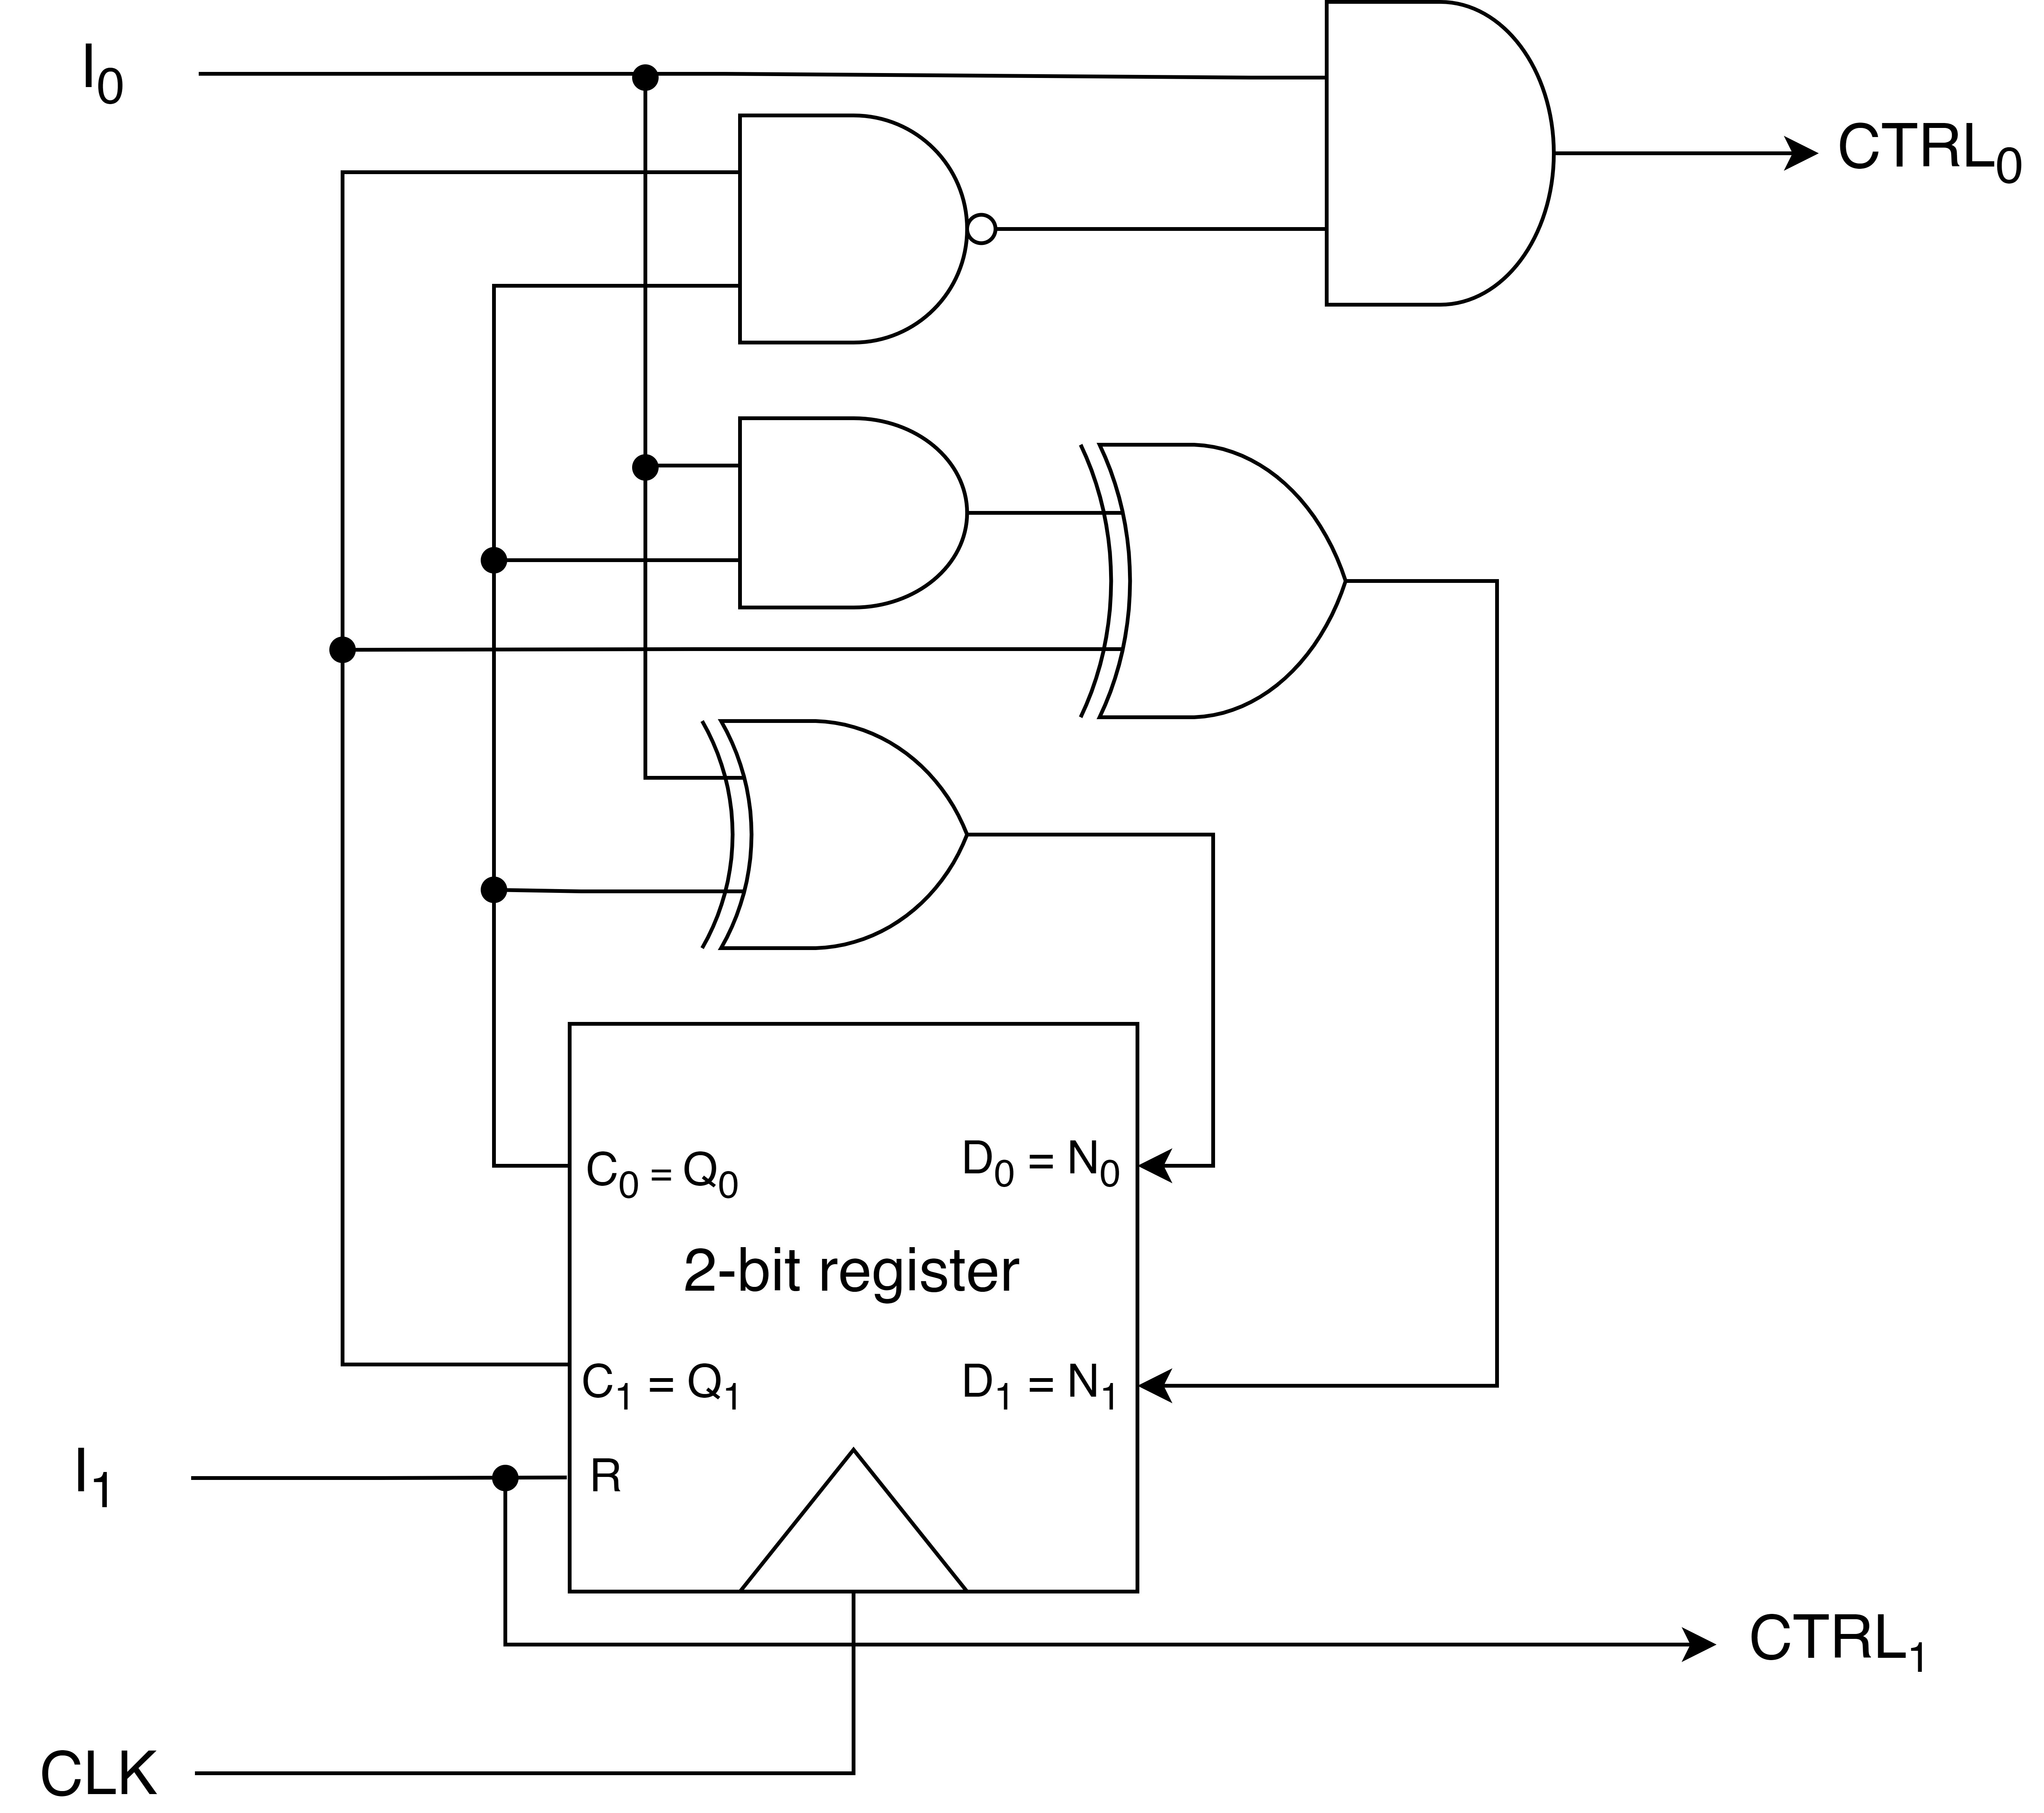
\includegraphics[width=0.6\textwidth]{Figures/logic diagram.png}
    \caption{FSM logic diagram}
    \label{fig:fsm_logic_diagram}
\end{figure}

\noindent
The registers used in this circuit is of the same design as the register described in \autoref{subsubsec:accumulator}.

\subsection{AIMSpice}
\label{subsec:aimspicemethod}

In the AIMSpice related part of the assignment, a 1 bit register, \autoref{fig:1-bit_reg}, will be implemented using the designs shown in \autoref{fig:dflipflop} and \ref{fig:setreset}.

\begin{figure}[H]
    \centering
    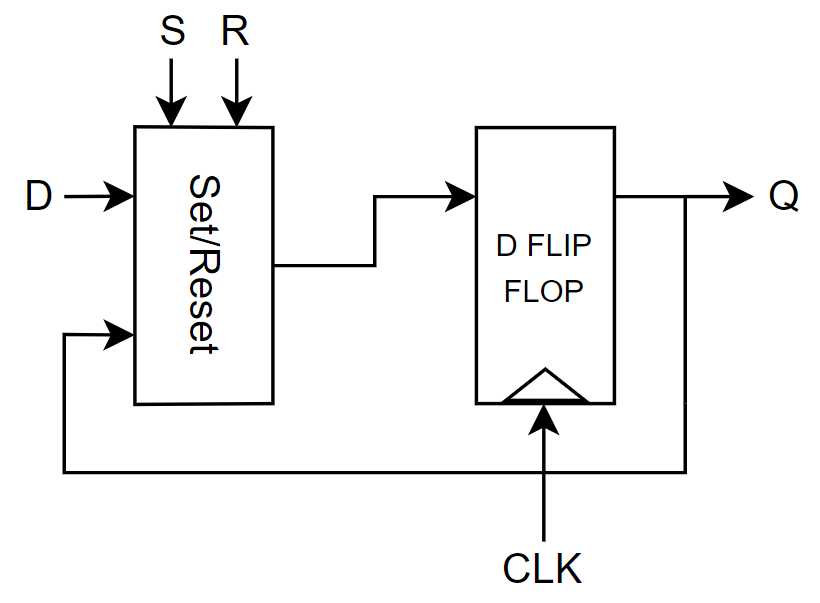
\includegraphics[width=0.6\textwidth]{Figures/1-bit register.png}
    \caption{1-bit register, with inputs Data, Reset and Set}
    \label{fig:1-bit_reg}
\end{figure}

To implement the register in AIMSpice, different logic gates are made using transistors. The different logic gates used in the 1-bit register are NOT-, AND- and transmission gates. This is shown in \autoref{fig:NOT} and \ref{fig:NAND}. To achieve a low static power consumption transistor stacking is used as that will give a lower leakage power. Through testing of different widths and lengths of the transistors, we found that a width of 100nm and a length of 300nm, gave the lowest leakage current while still having the correct functionality. 

\begin{figure}[H]
\centering
\begin{minipage}{0.4\textwidth}
    \centering
    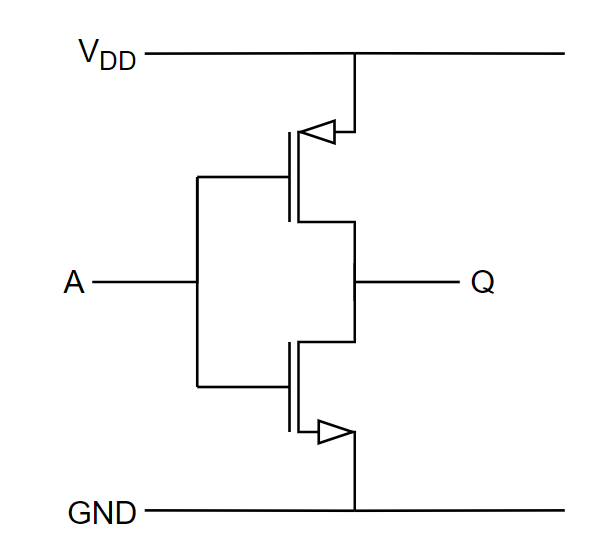
\includegraphics[width=\linewidth]{Figures/Not gate.png}
    \caption{\parbox{0.5\textwidth}{NOT-gate using MOSFET and transistor stacking}}
    \label{fig:NOT}
\end{minipage}
\begin{minipage}{0.4\textwidth}
    \centering
    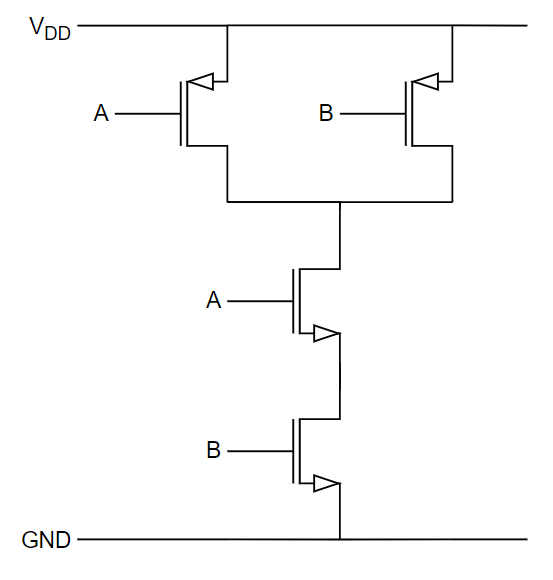
\includegraphics[width=0.9\linewidth]{Figures/Nand Gate.png}
    \caption{\parbox{0.5\textwidth}{NAND-gate using MOSFET and transistor stacking}}
    \label{fig:NAND}
\end{minipage}
\end{figure}

The AND gate is made by connecting a NAND and NOT in series, as shown in \autoref{fig:AND}.
\begin{figure}[H]
    \centering
    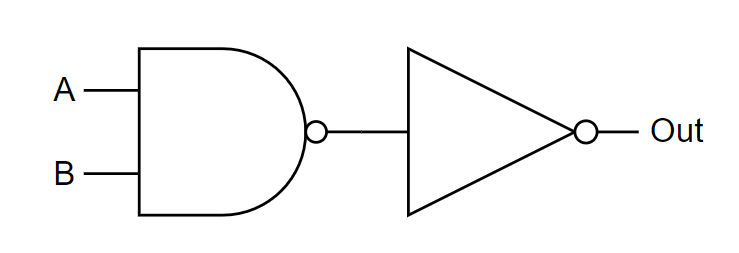
\includegraphics[width=0.4\linewidth]{Figures/And gate.png}
    \caption{AND gate}
    \label{fig:AND}
\end{figure}


\subsubsection{AIMSpice testing}
\label{subsubsec:aimspice_testing}
To test the 1-bit register made by in AIMSpice, we have to set some square waves for the clock signal, the data input, and the set and reset signals.

As shown in \autoref{fig:aimspice_pulses}, we use the PULSE function in AIMSpice to create square waves for the different inputs. These inputs will together determine what the output Q is set to.

\begin{figure}[H]
\centering
\begin{minipage}{0.9\textwidth}
\begin{lstlisting}[style=aimspiceStyle]
VD D 0 PULSE(0 C_VDD 25n RISE_TIME FALL_TIME 20ns 40ns)
VCLK CLK 0 PULSE(0 C_VDD 0 RISE_TIME FALL_TIME CLK_HIGH CLK_PERIOD)
VS S 0 PULSE(0 C_VDD 25n RISE_TIME FALL_TIME 60n 120n)
VR R 0 PULSE(0 C_VDD 145n RISE_TIME FALL_TIME 50n 100n)
\end{lstlisting}
\end{minipage}
\caption{AIMSpice code for creating square waves for the input signals, with all combinations of the inputs present.}
\label{fig:aimspice_pulses}
\end{figure}

The register should have the functionality as shown in the \autoref{tab:registerFunc}. Where the value of Q gets set to D if set is low and it keeps its previous value if set is high. If reset is high, the value Q is set to low. 

\begin{table}[H]
\centering
\caption{Functionality of 1bit-register}
\label{tab:registerFunc}
\begin{tabular}{|l|l|l|}
\cline{1-3}
\rowcolor[HTML]{C0C0C0} 
R & S & Q  \\ \cline{1-3}
0 & 0 & Q  \\ \cline{1-3}
0 & 1 & D  \\ \cline{1-3}
1 & 0 & 0  \\ \cline{1-3}
1 & 1 & 0  \\ \cline{1-3}
\end{tabular}
\end{table}


\subsection{Verilog}

In this section we create the subsystems and testbenches for them using the hardware descriptive language Verilog. A testbench for the full circuit is also created in this section.

\subsubsection{FSM in Verilog}
\label{subsec:fsm_verilog}

The FSM is implemented and its functionality is verified using Verilog. An excerpt of the logic part is given below in \autoref{fig:verilog_FSM_excerpt}. The complete code for implementing the FSM in Verilog is given in \autoref{verilog_FSM} in the appendix.


\begin{figure}[H]
\centering
\caption{Excerpt of the FSM implemented in Verilog.}
\label{fig:verilog_FSM_excerpt}
\begin{minipage}{0.33\textwidth}
\begin{lstlisting}[style=verilogStyle]
xor(N[0], C[0], RunIN);
and(A, C[0], RunIN);
xor(N[1], A, C[1]);
nand(B, C[0], C[1]);
and(RunOUT, B, RunIN);
\end{lstlisting}
\end{minipage}
\end{figure}


To simplify the implementation, the register is written as a separate module, shown in the appendix \autoref{verilog_onebitregister}.

To test the functionality, a separate testbench-module is made in verilog. The FSM is run through a series of different possible inputs. The output timing diagram is subsequently analyzed to verify that the FSM has the correct output based on the input.

\subsubsection{MAC in Verilog}
\label{subsubsec:MAC_in_verilog}

As the MAC is composed of three subcircuits, these are implemented, using the designs in \autoref{subsec:circuitDesign}, and tested with Verilog testbenches separately. All the code for the implementation of the subsystems are found in \autoref{appendix:Verilog-code}. 

The 2-bit multiplier and the 8-bit adder is set up to loop through all possible combinations of inputs and checked if the output matches what is expected. \autoref{fig:verilog_adderTB_excerpt} shows how to loop through the inputs on the adder.

\begin{figure}[H]
\centering
\caption{Loop to check all combinations for the adder.}
\label{fig:verilog_adderTB_excerpt}
\begin{minipage}{0.8\textwidth}
\begin{lstlisting}[style=verilogStyle]
for(Acount = 0 ; Acount < 256 ; Acount++) begin
    for(Bcount = 0 ; Bcount < 256 ; Bcount++) begin
        A = Acount;
        B = Bcount;
        #1;
        if((A+B) == S) begin
            $display(A,"+",B,"=",S);
        end else begin
            $display("Error: ", A, "+", B, "=",S);
            errors++;
        end
    end
end
\end{lstlisting}
\end{minipage}
\end{figure}

A and B are 8-bit input signals to the adder which can represent unsigned integers 0 to 255. Note the small delay needed for the signals to propagate the circuit. A similar approach can be used to verify the functionality of the multiplier and the register. 

For the register testbench, given in \autoref{verilog_registerTB}, one also has to account for the delay needed for the clock to have one rising edge before next input is tested. A testbench was also made for the MAC put together without the FSM. The procedure used for this testbench is the same as described in \autoref{subsubsec_FullMAC_verilog}. All testbenches can be found in \autoref{sec:verilog_testbenches}.

\subsubsection{Full MAC in Verilog}
\label{subsubsec_FullMAC_verilog}

Finally, to test the entire MAC put together the modules are put together as a complete circuit, shown in \autoref{verilog_fullmac}. A testbench is created to empirically test different combinations of inputs. As all combinations of current and previous inputs cannot easily be tested, like for the adder and multiplier isolated, the complete circuit is put through a series of randomized inputs A and B using the system function ''\$random''. The simulation can be repeated for different inputs by changing the variable ''randomSeed'' to a different integer.

\subsection{Must include}
The method section MUST INCLUDE:
\begin{itemize}
    \item One or more illustrations showing your circuit. As a minimum you must include one figure of the circuit at the logic gate level, and one of what you implemented at transistor level in AIMSpice.
    \item Figure showing the state diagram for your final state machine (FSM).
    \item Explanations of design choices you made when creating the circuit.
    \item Explanations of the simulations you did (not the results, just how they were done).
\end{itemize}
\section{Results}
\label{sec:results}

\subsection{AimSpice}

To test the 1-bit register made by in AimSpice, we have to set some square waves for the clock signal, the data input, and the set and reset signals.

As shown in appendix \ref{appendix:aimspice}, line 95-98, we use the PULSE function in AimSpice to create square waves for the different inputs. These inputs will together determine what the output Q is set to. 

The register could have different effect and operations due to the corner of the transistor and the temperature. There are five corners the transistors could be; TT(typical-typical), SS(slow-slow), FF(fast-fast), SF(slow-fast) and FS(fast-slow). For all of the corners they have been tested for three temperatures, 0$^\circ C$, 27$^\circ C$ and 70$^\circ C$. All the different plots for the different cases are shown in the appendix \ref{appendix:aimspicePlots}. 

To validate the functionality of the register, one can examine the plot of the TT and FF corner at 27$^\circ C$. 

The register should have the functionality as shown in the table \ref{tab:registerFunc}. Where the value of Q gets set to D if set is low and it keeps its previous value if set is high. If reset is high, the value Q is set to low. 

\begin{table}[H]
\label{tab:registerFunc}
\centering
\caption{Functionality of 1bit-register}
\begin{tabular}{|l|l|l|}
\cline{1-3}
R & S & Q  \\ \cline{1-3}
0 & 0 & Q  \\ \cline{1-3}
0 & 1 & D  \\ \cline{1-3}
1 & 0 & 0  \\ \cline{1-3}
1 & 1 & 0  \\ \cline{1-3}
\end{tabular}
\end{table}

\begin{figure}[H]
    \centering
    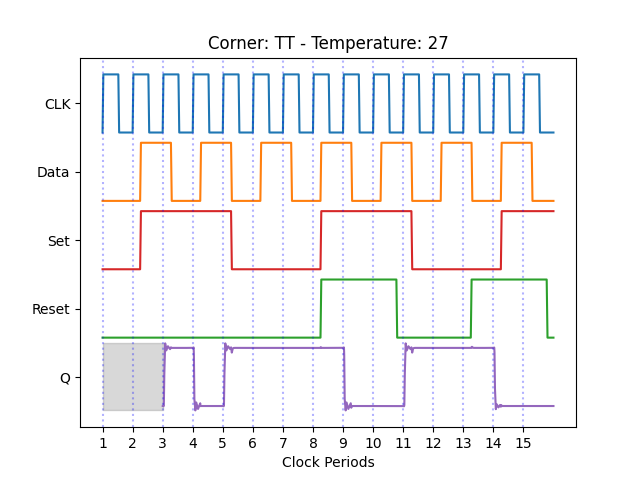
\includegraphics[width=\textwidth]{Figures/Aimspice_Plots/TT_27.png}
    \caption{Plot of register for TT corner}
    \label{fig:result_TT27}
\end{figure}

As shown in figure \ref{fig:result_TT27} and figure \ref{fig:result_FF27}, the different combinations of the inputs signals. If set is high, Q only updates to the D-value when the CLK changes from low to high. And if the reset is high, the value Q is overruled to low, even if set and D is high.

When looking at the different corners and temperatures, the difference of the functionality is quite similar. One can see in this case with the TT and FF corners at 27$^\circ C$, that the register is just a tiny fraction more stable with a FF corner rather than a TT corner.

\begin{figure}[H]
    \centering
    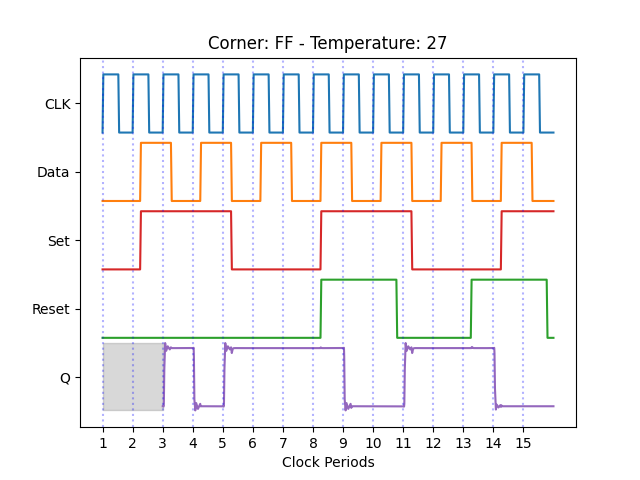
\includegraphics[width=\textwidth]{Figures/Aimspice_Plots/FF_27.png}
    \caption{Plot of register for FF corner}
    \label{fig:result_FF27}
\end{figure}

\subsubsection{Static Power Consumption}

We have therefore chosen a value for $V_{DD} = 0.85V$, as a lower $V_{DD}$ gives a lower power consumption. By using the function operating point in AimSpice, a current in the $V_{DD}$ node can be found.

Table \ref{tab:leakage} shows the different leakage current for the different corners with all three temperatures. To calculate the static power consumption, we use the formula \ref{eq:power} for all the values and get table \ref{tab:power}.

\begin{table}[H]
\centering
\caption{Leakage Current}
\label{tab:leakage}
\resizebox{\columnwidth}{!}{%
\begin{tabular}{llllll}
\cline{2-6}
\multicolumn{1}{l|}{} &
  \multicolumn{1}{l|}{TT} &
  \multicolumn{1}{l|}{SF} &
  \multicolumn{1}{l|}{FS} &
  \multicolumn{1}{l|}{SS} &
  \multicolumn{1}{l|}{FF} \\ \hline
\multicolumn{1}{|l|}{0 $^\circ$C} &
  \multicolumn{1}{l|}{10.764 nA} &
  \multicolumn{1}{l|}{7.576 nA} &
  \multicolumn{1}{l|}{27.658 nA} &
  \multicolumn{1}{l|}{5.667 nA} &
  \multicolumn{1}{l|}{31.842 nA} \\ \hline
\multicolumn{1}{|l|}{27 $^\circ$C} &
  \multicolumn{1}{l|}{23.828 nA} &
  \multicolumn{1}{l|}{83.146 $\mu$A} &
  \multicolumn{1}{l|}{58.765 nA} &
  \multicolumn{1}{l|}{13.360 nA} &
  \multicolumn{1}{l|}{67.994 nA} \\ \hline
\multicolumn{1}{|l|}{70 $^\circ$C} &
  \multicolumn{1}{l|}{64.986 nA} &
  \multicolumn{1}{l|}{64.437 nA} &
  \multicolumn{1}{l|}{151.939 nA} &
  \multicolumn{1}{l|}{33.104 nA} &
  \multicolumn{1}{l|}{176.953 nA} \\ \hline
 &  &  &  &  & 
\end{tabular}%
}
\end{table}

\begin{table}[H]
\centering
\caption{Static Power Consumption}
\label{tab:power}
\resizebox{\columnwidth}{!}{%
\begin{tabular}{llllll}
\cline{2-6}
\multicolumn{1}{l|}{} &
  \multicolumn{1}{l|}{TT} &
  \multicolumn{1}{l|}{SF} &
  \multicolumn{1}{l|}{FS} &
  \multicolumn{1}{l|}{SS} &
  \multicolumn{1}{l|}{FF} \\ \hline
\multicolumn{1}{|l|}{0 $^\circ$C} &
  \multicolumn{1}{l|}{9.1494 nW} &
  \multicolumn{1}{l|}{6.4396 nW} &
  \multicolumn{1}{l|}{23.509 nW} &
  \multicolumn{1}{l|}{4.8170 nW} &
  \multicolumn{1}{l|}{27.066 nW} \\ \hline
\multicolumn{1}{|l|}{27 $^\circ$C} &
  \multicolumn{1}{l|}{20.254 nW} &
  \multicolumn{1}{l|}{70.674 $\mu$W} &
  \multicolumn{1}{l|}{49.950 nW} &
  \multicolumn{1}{l|}{11,356 nW} &
  \multicolumn{1}{l|}{57.795 nW} \\ \hline
\multicolumn{1}{|l|}{70 $^\circ$C} &
  \multicolumn{1}{l|}{55.238 nW} &
  \multicolumn{1}{l|}{64.772 nW} &
  \multicolumn{1}{l|}{129.15 nW} &
  \multicolumn{1}{l|}{28.138 nW} &
  \multicolumn{1}{l|}{159.41 nW} \\ \hline
 &  &  &  &  & 
\end{tabular}%
}
\end{table}

Since the intrinsic concentration, , is a strong function of temperature (it approximately doubles for every
temperature increase of 11 °C for silicon), the leakage current is also a strong function of temperature. The leakage
current roughly doubles for every 11 °C rise in temperature; thus, at higher temperatures it is much larger than at
room temperature.

\subsection{Verilog}

In this subsection results of Verilog-simulation will be presented. All Verilog-code is given in appendix~\ref{appendix:Verilog-code}.

Figure~\ref{fig:fsm_simulation} shows the FSM simulated for randomized inputs $I_1$ and $I_0$.

\begin{figure}[H]
    \centering
    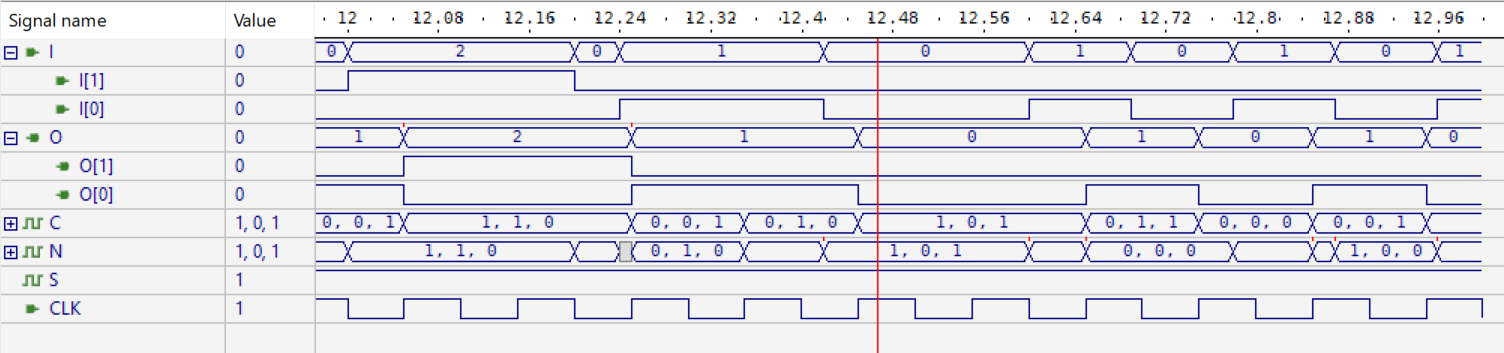
\includegraphics[width=\textwidth]{Figures/Test of FSM.png}
    \caption{Timing diagram of FSM simulated in Verilog}
    \label{fig:fsm_simulation}
\end{figure}

From the figure we see that the memory transitions to the expected states based on the inputs. The FSM begins in state ''Run-1'' and transitions to state ''Reset'' as the reset input $I_1$ is set high. The next state is ''Run-1'', then ''Run-2''. The Run-bit $I_0$ is then set low, resulting in a two-period pause in state ''Pause-2''. Further the FSM transitions to ''Run-3'', ''Pause'' and ''Run-1''.

This simulation was run and verified to follow the wanted behaviour as given by table~\ref{tab:truthtable}.

Figure~\ref{fig:eightbitadder_sim} shows a simulation of the 8-bit adder with random 8-bit inputs A and B. Note that all values in the timing diagram are hexadecimal and that any overflow-bits are handled outside our system. The code used for this simulation is given in listing~\ref{verilog_8bitadder}.

\begin{figure}[H]
    \centering
    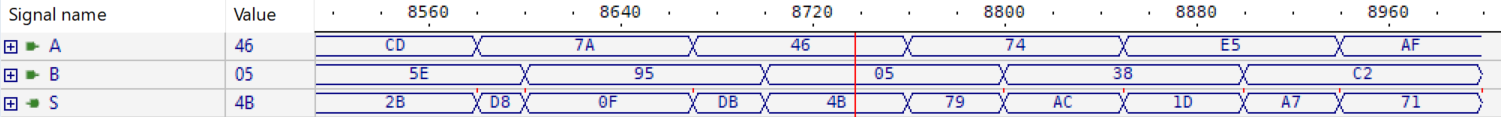
\includegraphics[width=\textwidth]{Figures/Test of eightbitadder.png}
    \caption{Timing diagram of 8-bit adder simulated in Verilog}
    \label{fig:eightbitadder_sim}
\end{figure}

Figure~\ref{fig:dflipflop_sim} shows a simulation of a single D Flip-Flop realized in Verilog.

\begin{figure}[H]
    \centering
    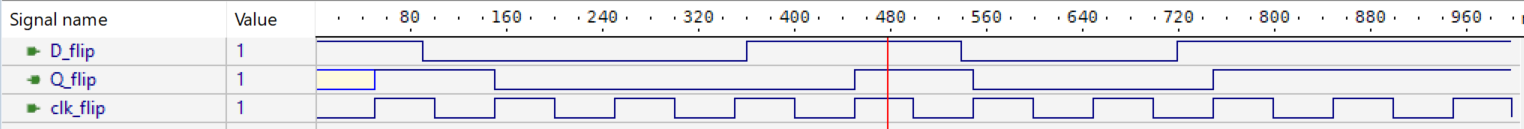
\includegraphics[width=\textwidth]{Figures/Test of Dflipflop.png}
    \caption{Timing diagram of D Flip-Flop simulated in Verilog}
    \label{fig:dflipflop_sim}
\end{figure}

Figure \ref{fig:8bitregister_sim} shows a simulation of a 8-bit register realized in Verilog.

\begin{figure}[H]
    \centering
    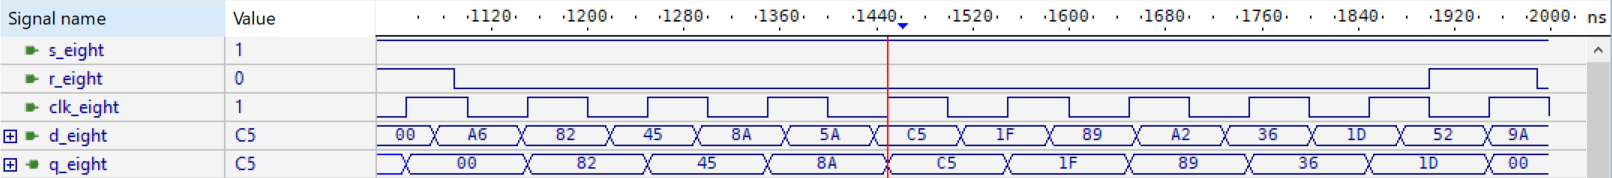
\includegraphics[width=\textwidth]{Figures/VerilogPlot_8bitreg.png}
    \caption{Timing diagram of an 8-bit register simulated in Verilog}
    \label{fig:8bitregister_sim}
\end{figure}

Figure~\ref{fig:multiplier_sim} shows a simulation of the 2-bit multiplier realized in Verilog. Inputs A and B are stimulated with arbitrary two bit values to observe the possible outputs. The multiplier has a 4-bit output as the largest possible output result, 9, needs four bits to be represented in binary.

\begin{figure}[H]
    \centering
    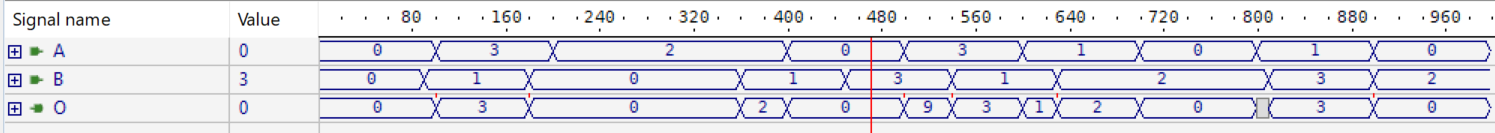
\includegraphics[width=\textwidth]{Figures/Test of multiplier.png}
    \caption{Timing diagram of multiplier simulated in Verilog}
    \label{fig:multiplier_sim}
\end{figure}



% Present the results of your simulations in this section. Use tables and graphs or other figures to illustrate your results. Remember: The table caption goes above the table, the figure caption goes below the figure.

% The results section must include:
% \begin{itemize}
%     \item Figures and/or tables that show the results of your simulation.
%     \item Text that describe what we see in the simulation results (e.g. as expected we can see that XYZ which means the circuit functions as intended).
%     \item NB! The result section is a \textit{what?}-section. \textit{What} where the results? \textit{What} do the figures/results mean? Any \textit{why}-questions you might want to write about and try to answer typically belong in the discussion section.
% \end{itemize}
\section{Discussion}
\label{sec: Discussion}

\subsection{Design improvements}

Some thoughts following the project have emerged about design choices that could have been made different. One consideration is that the 8-bit adder's four most significant bits strictly speaking does not need to be full adders as one of the inputs for these bits always will be zero. A change that would simplify the FSM is using the run input signal as the set-bit on the state register. This would simplify the next-state logic as it only would need to increment the current state.

Were we to prioritize the dynamic power consumption, one could consider disabling the clock for the MAC part of the circuit. If the circuit is expected to be in the non-operating state for longer periods of time, one could also consider implementing power gating, i.e. disabling $V_{DD}$ for specific parts of the circuit.

\subsection{AIMSpice}

When looking at the different corners and temperatures, there is some differences in the stability when the Q-value changes state. 

One can see in the case, \autoref{fig:TT_diffTemps}, with the TT corner at the different temperatures, that the register is just a tiny fraction more stable with a at higher temperatures when Q changes from low to high. When Q goes high to low with the TT corner, the lower temperature has little to none ripple, while the higher temperature is more unstable. 

For the case where we look at the different corners at the same temperature, \autoref{fig:27_diffCorners}, it is shown that when Q goes from low to high the TT, FF and SF corners have the most ripples while the SS and FS corner have the least ripple. When Q changes from high to low all corners at 27$^\circ$C have quite similar ripple. 

As shown in \autoref{fig:result_TT27}, one can see that there is a small dip in the Q-signal. This is due to the Set signal changing from high to low. We don't know why this happens, but we can assume that it's because of the change of the output in the control circuit from new data (D) to stored data (Q).

When we look at the static power consumption, \autoref{tab:power}, and compare it to \autoref{eq:power}, one can see that the static power consumption will increase with the temperature. This is in line with what is expected. The FF corner also gives a higher static power consumption than the TT corner, which is to be expected due with a lower threshold voltage and therefore higher $V_{eff}$.

\subsection{Verilog}

The Verilog simulations show that the design works as intended according to \autoref{tab:specifications}.
An interesting observation regarding the FSM is the fact that even though the FSMs state only updates on the positive edge of the clock, the control signal is free to change at other times, depending on the FSMs input. This is because the FSM is a Mealy machine. Nonetheless, this behaviour does not affect the function of the MAC receiving the control signal as it only operates on the positive edge.

Another observation is that \textit{when} the control signal changes on a rising edge, what operation the MAC performs is dependent on what value the control signal held \textit{before} it changed. From the timing diagram in \autoref{fig:fullmac_simulation}, we see that it is not always obvious by the output Y what is going on inside the circuit. E.g. pausing the MAC would do the same as having A or B equal to 0. For this reason it is a good idea to observe the control signal while verifying the functionality of the entire circuit. 

The adder is, as expected, limited by its number of bits in how large numbers it is able to represent. Resultingly, when the actual sum of the numbers is larger than 255, the most significant bit will overflow and the output is becomes the sum decremented by 256.










% Discuss your results. You presented your results in the last section, so you do not need to repeat everything here. Just focus on the most interesting results and discuss these.

% Was there anything unexpected or weird about your results? What are possible explanations for these observations? It is good to draw on theory. This section and the theory section are the sections where it is natural to have the most references to literature (papers, the book, other).

% The discussion section must include a discussion of your results:
% \begin{itemize}
%     \item If the circuit did not work properly, \textit{why} might that be? 
%     \item Did some of your results turn out differently than you expected. \textit{Why}? You do not have to come to a definite answer, but should try to discuss at least one possible explanation.
%     \item It could be interesting to discuss the choices you made to reduce static power consumption, and potential improvements to these.
% \end{itemize}
\section{Conclusion}
\label{sec:conclution}

Make some concluding remarks. The length of this section should be somewhere between a paragraph and a page.

The conclusion should include your key findings. Make the conclusion as concrete as possible by using numbers for the result (e.g. what was the static power consumption at a given supply voltage).

\newpage
\addcontentsline{toc}{section}{References}
\bibliographystyle{unsrt}
\bibliography{bibliography}

\newpage
\vspace*{7 cm}
\begin{center}
\textbf{\Huge Appendices}
\end{center}
\addcontentsline{toc}{section}{Appendices}
\appendix
\section{AIMSpice Code}
\label{appendix:aimspice}

\begin{lstlisting}[style=aimspiceStyle, caption=1-bit register in AIMSPICE, label=testcode]
**************************************************************
* Including the file containing the NMOS and PMOS transistors
.include gpdk90nm_tt.cir
**************************************************************

**************************************************************
.PARAM W_VAL=150n
.PARAM L_VAL=300n
**************************************************************

**************************************************************
* Subcircuit for a NOT gate 
.subckt NOT GND VDD A OUT
XMP1 OUT A VDD VDD PMOS1V W=W_VAL L=L_VAL 
XMN1 OUT A GND GND NMOS1V W=W_VAL L=L_VAL
.ends NOT
**************************************************************

**************************************************************
* Subcircuit for a NAND gate 
.subckt NAND GND VDD A B OUT
XMP1 VDD A OUT VDD PMOS1V W=W_VAL L=L_VAL 
XMP2 VDD B OUT VDD PMOS1V W=W_VAL L=L_VAL 
XMN1 OUT A C C NMOS1V W=W_VAL L=L_VAL 
XMN2 C B GND GND NMOS1V W=W_VAL L=L_VAL 
.ends NAND
**************************************************************

**************************************************************
* Subcircuit for an AND gate 
.subckt AND GND VDD A B OUT
XAND1 GND VDD A B C NAND
XNOT1 GND VDD C OUT NOT
.ends AND
**************************************************************

**************************************************************
* Subcircuit for a NOR gate 
.subckt NOR GND VDD A B OUT
XMP1 VDD A C VDD PMOS1V W=W_VAL L=L_VAL 
XMP2 C B OUT C PMOS1V W=W_VAL L=L_VAL 
XMN1 OUT B GND GND NMOS1V W=W_VAL L=L_VAL 
XMN2 OUT A GND GND NMOS1V W=W_VAL L=L_VAL 
.ends NOR
**************************************************************

**************************************************************
* Subcircuit for an OR gate 
.subckt OR GND VDD A B OUT
XGATENOR1 GND VDD A B C NOR
XNOT1 GND VDD C OUT NOT
.ends OR
**************************************************************

**************************************************************
* Subcircuit for a TRANSMISSION gate 
.subckt TRANS GND VDD IN EN_N EN_P OUT
XMN1 IN EN_N OUT GND NMOS1V W=W_VAL L=L_VAL
XMP1 IN EN_P OUT VDD PMOS1V W=W_VAL L=L_VAL 
.ends TRANS
**************************************************************

**************************************************************
* Subcircuit for a MUX for set and reset
.subckt MUX GND VDD S R DI Q DO
XNOT1 GND VDD S 1 NOT
XTRANS1 GND VDD DI S 1 2 TRANS
XTRANS2 GND VDD Q 1 S 2 TRANS
XNOT2 GND VDD R 3 NOT
XAND GND VDD 2 3 DO AND
.ends 
**************************************************************

**************************************************************
*Subcircuit for a D FLIP FLOP using TRANSMITION gates 
.subckt FLOP GND VDD CLK D Q 
XNOT1 GND VDD D 1 NOT
XNOT_CLK GND VDD CLK NOTCLK NOT
XTRANS1 GND VDD 1 NOTCLK CLK 2 TRANS
XNOT2 GND VDD 2 3 NOT
XNOT3 GND VDD 3 4 NOT 
XTRANS2 GND VDD 4 CLK NOTCLK 2 TRANS
XTRANS3 GND VDD 3 CLK NOTCLK 5 TRANS
XNOT4 GND VDD 5 6 NOT
XNOT5 GND VDD 6 7 NOT
XTRANS4 GND VDD 7 NOTCLK CLK 5 TRANS
XNOT6 GND VDD 6 Q NOT
.ends
**************************************************************

**************************************************************
* Subcircuit for 1bit register with set and reset
.subckt REGISTER GND VDD CLK S R D Q 
XMUX1 GND VDD S R D Q 1 MUX
XFLOP GND VDD CLK 1 Q FLOP
.ends
**************************************************************


**************************************************************
.PARAM RISE_TIME=0.1n 
.PARAM FALL_TIME=0.1n 
.PARAM CLK_PERIOD=20n 
.PARAM CLK_HIGH=10n 
.PARAM V_DD=0.85


*Setting VDD = 1, the CLK and D as two different pulses
VDD 1 0 V_DD
VD D 0 PULSE(0 V_DD 25n RISE_TIME FALL_TIME 20ns 40ns)
VCLK CLK 0 PULSE(0 V_DD 0 RISE_TIME FALL_TIME CLK_HIGH CLK_PERIOD)
VS S 0 PULSE(0 V_DD 35n RISE_TIME FALL_TIME 60n 120n)
VR R 0 PULSE(0 V_DD 145n RISE_TIME FALL_TIME 50n 100n)
**************************************************************

**************************************************************
*Defining the register
XREG 0 1 CLK S R D Q REGISTER
**************************************************************

**************************************************************
*Plotting D, CLK and Q for the register
.plot v(Q)
.plot v(D)
.plot v(CLK)
.plot v(S) 
.plot v(R)
**************************************************************

\end{lstlisting}


\section{Verilog Code}

\begin{lstlisting}[style=verilogStyle, caption=D Flip-Flop in Verilog, label=verilog_dflipflop]
module D_Flip_Flop ( input D_flip , output Q_flip , input clk_flip );
	
	wire clk_bar_flip; 
	not(clk_bar_flip, clk_flip);
	not(w1_flip, D_flip);	  
	wire w2_flip;
	cmos(w2_flip, w1_flip, clk_bar_flip, clk_flip);	
	wire w3_flip;
	not(w3_flip, w2_flip); 
	wire w4_flip;
	not(w4_flip, w3_flip);
	cmos(w2_flip, w4_flip, clk_flip, clk_bar_flip);	 
	wire w5_flip;
	cmos(w5_flip, w3_flip, clk_flip, clk_bar_flip);
	wire w6_flip, w7_flip;
	not(w6_flip, w5_flip);
	not(w7_flip, w6_flip);
	cmos(w5_flip, w7_flip, clk_bar_flip, clk_flip);	 
	not(Q_flip, w6_flip);

endmodule
\end{lstlisting}

\begin{lstlisting}[style=verilogStyle, caption=Set/Reset-Circuit in Verilog, label=verilog_regmux]
module Reg_mux (
    input S_mux,
    input R_mux,
    input D_I_mux,
    input Q_mux,
    output D_O_mux
);			  
wire Y_mux;	
assign sbar = ~S_mux;
assign rbar = ~R_mux;  

cmos(Y_mux,D_I_mux, S_mux, sbar);
cmos(Y_mux,Q_mux,sbar,S_mux);
and(D_O_mux, rbar, Y_mux);

endmodule  
\end{lstlisting}

\begin{lstlisting}[style=verilogStyle, caption=1-bit Register in Verilog, label=verilog_1bitregister]
`include "Reg_mux.v"
`include "D_Flip_Flop.v"

module onebit_register (input D, input S, input R, input CLK, output Q);

  wire D_O_mux; // Output from the multiplexer 

  Reg_mux mux_instance (
    .S_mux(S),
    .R_mux(R),
    .D_I_mux(D), 
    .Q_mux(Q), // Connect the Q output of the flip-flop to the input of the multiplexer  
    .D_O_mux(D_O_mux)
  );

  D_Flip_Flop flip_flop_instance (
    .D_flip(D_O_mux), // Connect the input of the flip-flop to the multiplexer's output
    .Q_flip(Q),
    .clk_flip(CLK)
  );  
  
  not(D, Q);

endmodule
\end{lstlisting}

\begin{lstlisting}[style=verilogStyle, caption=8-bit Register in Verilog, label=verilog_8bitregister]
`include "onebit_register.v"
module eightbit_register ( input s_eight , input r_eight ,input clk_eight, input [7:0] d_eight ,output [7:0] q_eight );
	
	wire [7:0] q_onebit[7:0];
	
	onebit_register onebit_instance0 (
	    .S(s_eight),
	    .R(r_eight),
		.CLK(clk_eight),
	    .D(d_eight[0]), // Connect the corresponding bit of d_eight to onebit_register
	    .Q(q_eight[0])
	); 
	onebit_register onebit_instance1 (
	    .S(s_eight),
	    .R(r_eight),
		.CLK(clk_eight),
	    .D(d_eight[1]), // Connect the corresponding bit of d_eight to onebit_register
	    .Q(q_eight[1])
	);
	onebit_register onebit_instance2 (
	    .S(s_eight),
	    .R(r_eight),
		.CLK(clk_eight),
	    .D(d_eight[2]), // Connect the corresponding bit of d_eight to onebit_register
	    .Q(q_eight[2])
	);		   
	onebit_register onebit_instance3 (
	    .S(s_eight),
	    .R(r_eight),
		.CLK(clk_eight),
	    .D(d_eight[3]), // Connect the corresponding bit of d_eight to onebit_register
	    .Q(q_eight[3])
	);
	onebit_register onebit_instance4 (
	    .S(s_eight),
	    .R(r_eight),
		.CLK(clk_eight),
	    .D(d_eight[4]), // Connect the corresponding bit of d_eight to onebit_register
	    .Q(q_eight[4])
	);
	onebit_register onebit_instance5 (
	    .S(s_eight),
	    .R(r_eight),
		.CLK(clk_eight),
	    .D(d_eight[5]), // Connect the corresponding bit of d_eight to onebit_register
	    .Q(q_eight[5])
	);
	onebit_register onebit_instance6 (
	    .S(s_eight),
	    .R(r_eight),
		.CLK(clk_eight),
	    .D(d_eight[6]), // Connect the corresponding bit of d_eight to onebit_register
	    .Q(q_eight[6])
	);
	onebit_register onebit_instance7 (
	    .S(s_eight),
	    .R(r_eight),
		.CLK(clk_eight),
	    .D(d_eight[7]), // Connect the corresponding bit of d_eight to onebit_register
	    .Q(q_eight[7])
	);

endmodule
\end{lstlisting}

\begin{lstlisting}[style=verilogStyle, caption=Half Adder in Verilog, label=verilog_halfadder]
module Half_Adder ( A_0 ,B_0 ,S_0 ,C_0 );

input A_0 ;
wire A_0 ;
input B_0 ;
wire B_0 ;
output S_0 ;
wire S_0 ;
output C_0 ;
wire C_0 ;

and(C_0, A_0, B_0);
xor(S_0, A_0, B_0);

endmodule
\end{lstlisting}

\begin{lstlisting}[style=verilogStyle, caption=Full Adder in Verilog, label=verilog_fulladder]
module Full_Adder ( C_I ,S_O ,A_I ,C_O ,B_I );

input C_I ;
wire C_I ;
output S_O ;
wire S_O ;
input A_I ;
wire A_I ;
output C_O ;
wire C_O ;
input B_I ;
wire B_I ;

wire w1,w2,w3;
xor(w1, A_I, B_I);
and(w2, A_I, B_I); 
and(w3, w1, C_I);
xor(S_O, w1, C_I);
or(C_O, w2, w3); 

endmodule
\end{lstlisting}

\begin{lstlisting}[style=verilogStyle, caption=8-bit Adder in Verilog, label=verilog_8bitadder]
`include "Half_Adder.v"
`include "Full_Adder.v"

module eightbit_adder (
    input [7:0] A,
    input [7:0] B,
    output [7:0] S
);

wire [7:0] carry;
wire [7:0] carry_out;

Half_Adder ha_instance_0 (
    .A_0(A[0]),
    .B_0(B[0]),
    .S_0(S[0]),
    .C_0(carry[0])
);

Full_Adder FA_1 (
    .A_I(A[1]),
    .B_I(B[1]),
    .C_I(carry[0]),
    .S_O(S[1]),
    .C_O(carry_out[1])
);

Full_Adder FA_2 (
    .A_I(A[2]),
    .B_I(B[2]),
    .C_I(carry_out[1]),
    .S_O(S[2]),
    .C_O(carry_out[2])
);

Full_Adder FA_3 (
    .A_I(A[3]),
    .B_I(B[3]),
    .C_I(carry_out[2]),
    .S_O(S[3]),
    .C_O(carry_out[3])
);

Full_Adder FA_4 (
    .A_I(A[4]),
    .B_I(B[4]),
    .C_I(carry_out[3]),
    .S_O(S[4]),
    .C_O(carry_out[4])
);

Full_Adder FA_5 (
    .A_I(A[5]),
    .B_I(B[5]),
    .C_I(carry_out[4]),
    .S_O(S[5]),
    .C_O(carry_out[5])
);

Full_Adder FA_6 (
    .A_I(A[6]),
    .B_I(B[6]),
    .C_I(carry_out[5]),
    .S_O(S[6]),
    .C_O(carry_out[6])
);

Full_Adder FA_7 (
    .A_I(A[7]),
    .B_I(B[7]),
    .C_I(carry_out[6]),
    .S_O(S[7]),
    .C_O(carry_out[7])
);

endmodule
\end{lstlisting}

\begin{lstlisting}[style=verilogStyle, caption=FSM in Verilog, label=verilog_fsm]
`include "D_Flip_Flop.v"

module FSM ( I ,CLK ,O );

//Initiate inputs+outputs

input [1:0] I ;
wire [1:0] I ;
input CLK ;
wire CLK ;
output [1:0] O ;
wire [1:0] O ;


//Initiate all internal wires

wire C[2:0];		//Current state		   
wire N[2:0];		//Next state   

wire C2not;
wire C1not;
wire C0not;
wire I1not;
wire I0not;
wire C0orC1;   
wire C1xorC0;
wire A;
wire B;
wire T;
wire D;
wire E;
wire F;
wire G;
wire H;
wire J;
wire K;	
wire S;	   //Set bit for testing
wire X;
wire Y;
wire Z;

	//Initiate the 3-bit register

	D_Flip_Flop flip_flop_instance_0 (
	.D_flip(N[0]),
	.Q_flip(C[0]),
	.clk_flip(CLK)
	);	  
	
	D_Flip_Flop flip_flop_instance_1 (
	.D_flip(N[1]),
	.Q_flip(C[1]),
	.clk_flip(CLK)
	);	
	
	D_Flip_Flop flip_flop_instance_2 (
	.D_flip(N[2]),
	.Q_flip(C[2]),
	.clk_flip(CLK)
	);	
	
	//Initiate the output logic
	
	and(O[1],C[1],C[2]);
	and(O[0],C0orC1,C2not);
	or(C0orC1, C[0], C[1]);
	
	
	//Initiate the Next state logic
	
	//NOT-gates
	not(C2not, C[2]);
	not(C1not, C[1]);
	not(C0not, C[0]);
	not(I1not, I[1]);
	not(I0not, I[0]);
	
	//other gates

	and(N[2], X, S);	//To initiate the register for simulation we make the next state N[2:0]=000 if S=0
	
	or(X, I[1], A, B);
	and(A, C[2], C1not, I0not);
	and(B, I0not, C2not, C1xorC0);
	xor(C1xorC0, C[1], C[0]);

	and(N[1], Y, S);	
	
	or(Y, I[1], T, D);
	and(T, C[2], C1not, I[0]);
	and(D, I[0], C2not, C1xorC0);
	
	and(N[0], Z, S);
	
	or(Z, K, J);	 
	or(K, G, H);
	or(J, E, F);	
	and(E, C2not, C0not, I1not, I[0]);
	and(F, C[2], C1not, C[0], I1not);
	and(G, C[1], C0not, I1not, I[0]);
	and(H, C2not, C[1], C0not, I1not);

endmodule
\end{lstlisting}

\begin{lstlisting}[style=verilogStyle, caption=, label=]
\end{lstlisting}

\section{Optional (rename based on what you put here)}
Sometimes one might end up running a lot of simulations, and then find out that not all of them were relevant enough to present in the actual report. Additional figures and results can then be included here (with a brief explanation so that the reader knows what they are looking at). This section of the appendix is optional, and might not be relevant for your group. 

Anything added here will not affect the grade directly, but might contribute to the overall impression of the work you have done (which is part of what we grade). Your grade will NOT be affected negatively if only the AIMSpice and Verilog code is in the appendix.
\end{document}
